\documentclass[es,apuntes]{uah}

\usepackage{subfigure}
\usepackage{amssymb}

\tema{2}
\titulo{Codificación de canal}{Lesson title}
%
\begin{document}

\titulacion{Optativa GIEC y GIT}
\departamento{Teoría de la Señal y Comunicaciones}
\asignatura{Comunicaciones Digitales}{}
\curso{2020/2021} % Do not show year

\maketitle


%%%%%%%%%%%%%%%%%%%%%%%
\section{Introducción}
%%%%%%%%%%%%%%%%%%%%%%%

El objetivo principal de un sistema de comunicaciones digital es transmitir un mensaje desde una fuente a un receptor a través de un determinado canal. Un codificador de canal tiene como objetivo encontrar la forma de representar el mensaje de forma que se consiga una transmisión libre de errores aunque el canal sea ruidoso. 

En principio parece claro que la única forma de conseguir este objetivo es restringir los mensajes que se envían por el canal, de forma que éstos sean tan solo un subconjunto de todos los mensajes posibles. Esta idea se muestra en la Figura \ref{fig:CodificacionDeCanal}. Como se puede observar, en el primer caso, se utiliza un alfabeto de 4 mensajes con 2 bits. Cualquier mensaje que recibamos es, en principio, válido, por lo que no nos es posible saber si se ha producido algún error. 

En el segundo caso, por otra parte, se introduce un codificador de canal que lo que hace es añadir un bit al mensaje transmitido, haciendo que, aunque haya 8 mensajes posibles con 3 bits, sólo 4 son válidos. Así, si recibimos un mensaje no válido sabremos con seguridad que se ha producido algún error en la transmisión, y podremos tomar las medidas oportunas. 


\begin{figure*}
	\centering
	\subfigure{\label{fig:CodificacionDeCanal1}\centering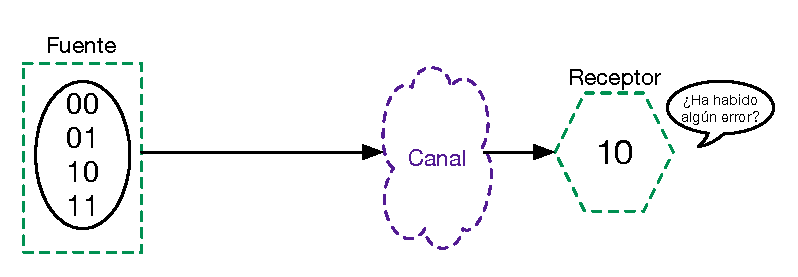
\includegraphics[width=12cm]{./Figuras/CodificacionDeCanal1}}\\
	\subfigure{\label{fig:CodificacionDeCanal2}\centering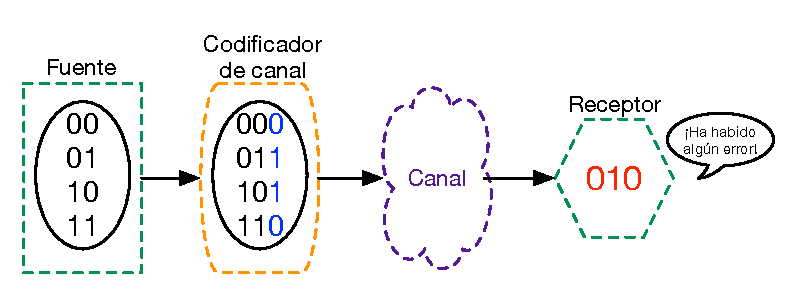
\includegraphics[width=12cm]{./Figuras/CodificacionDeCanal2}}
		\caption{Esquema de un sistema de comunicaciones digitales \subref{fig:CodificacionDeCanal1} sin codificación de canal y \subref{fig:CodificacionDeCanal2} con un codificador de canal que añade un bit extra. }	
		\label{fig:CodificacionDeCanal}
\end{figure*}

Debemos distinguir aquí dos tipos de sistemas distintos: {\bf sistemas detectores de errores} y {\bf sistemas correctores de errores}. Los primeros son, como se puede suponer, más sencillos de implementar que los segundos, y pueden aprovecharse de la posible existencia de un canal de retorno para que el receptor solicite la retransmisión de aquella información en la que se han detectado errores. Este tipo de sistemas son típicos en sistemas como por ejemplo redes de ordenadores. 

En otros casos la retransmisión de la información no es posible o no resulta práctica. Trataremos entonces de técnicas de corrección de errores. 

Empezaremos viendo algunos ejemplos de códigos muy simples que nos permitirán empezar a comprender las ideas básicas del problema para centrarnos después en los dos grandes tipos de codificadores de canal: los códigos bloque y los códigos convolucionales. 


%%%%%%%%%%%%%%%%%%%%%%%%%%%%%%%%
\section{Códigos de repetición}\index{Códigos de Repetición}\index{Repetición, Códigos de}
%%%%%%%%%%%%%%%%%%%%%%%%%%%%%%%%

Quizás la forma más sencilla de construir un código de protección frente a errores es repetir directamente cada bit $n$ veces, de forma que cada palabra código constará de $n$ bits idénticos. Esto no deja de ser lo mismo que hacemos nosotros cuando intentamos mantener una conversación en un ambiente muy ruidoso: repetir las cosas más de una vez. 

 Imaginemos por ejemplo que construimos un código de triple repetición con las palabras código \bits{000} y \bits{111}. Cualquier otra palabra recibida (p.ej. \bits{101} o \bits{010}) nos indica que se ha producido algún error. Este código tan simple nos permite tanto detectar como corregir errores, en función de cómo sea la implementación del decodificador:
 
 \begin{itemize}
 	\item Si sólo queremos detectar errores, basta con marcar cualquier palabra recibida distinta de las dos permitidas \bits{000} y \bits{111} y solicitar que se reenvíe.
 	\item Para corregir errores se puede utilizar una regla de mayoría, suponiendo que habrá menos bits erróneos que correctos en la palabra. Así, \bits{101} se decodificará como \bits{111} y \bits{010} como \bits{000}. Es interesante darse cuenta de que este sistema es capaz de corregir correctamente palabras con un error, pero si hay dos o tres errores se va a equivocar. 
 \end{itemize}
 
 En este caso vemos que hemos construido un codificador que, para cada bit de entrada ($k=1$) produce $n$ bits a la salida (en nuestro ejemplo $n=3$). Esto nos da una medida de la eficiencia del codificador, y así se define la {\bf tasa de codificación}\index{Tasa de codificación!Definición} como:
 
 \begin{displaymath}
 	R_c \triangleq \frac{k}{n}
 \end{displaymath}
 
 Otro parámetro que podemos definir a partir de lo visto para este codificador es la {\bf distancia mínima}\index{Distancia mínima de un código} de un código, que se define como la distancia Hamming más pequeña existente entre dos palabras código válidas. 
 
 La {\bf distancia Hamming}\index{Distancia Hamming} entre dos vectores, $d(\mathbf{x}, \mathbf{y})$, se calcula como el número de elementos distintos entre los dos vectores. Así, por ejemplo, si $\mathbf{x} = (\mathtt{1 0 1})$ e $\mathbf{y} = (\mathtt{0 0 1})$, entonces $d(\mathbf{x},\mathbf{y}) = 1$ ya que sólo el primer elemento es diferente entre ambos.  
 
 Para nuestro ejemplo de codificador de repetición podemos ver que se cumple que $d_{min} = 3$. La utilidad de la distancia mínima es que nos permite deducir cuál va a ser la capacidad de un determinado código en cuanto a la detección y/o corrección de errores. En concreto, si un código posee una distancia minima $d_{min}$, entonces

\begin{itemize}
	\item Podremos detectar no más de $d_{min}-1$ errores por palabra.
	\item Podremos corregir no más de $\frac{d_{min}-1}{2}$ errores por palabra.
%	\item Podremos detectar hasta $D$ errores por palabra si $d_{min} \geq D+1$.
%	\item Podremos corregir hasta $C$ errores por palabra si $d_{min} \geq 2C + 1$.
%	\item Podremos corregir $C$ errores y detectar $D>C$ errores por palabra si $d_{min} > C + D + 1$.
\end{itemize} 

 En nuestro caso, con $d_{min}=3$ podemos ver que es posible detectar hasta $2$ errores por palabra y corregir $1$ error, lo cual coincide con lo que ya habíamos deducido anteriormente.
 
 Supongamos ahora que el canal de transmisión utilizado hace que la probabilidad de que ocurra un error es $p_e \ll 1$. Es posible demostrar que la probabilidad de que ocurran $i$ errores en una palabra código de $n$ bits viene dada por:
 
 \begin{displaymath}
 	P(i,n) = \left ( \begin{array}{c}n \\i \end{array} \right ) \cdot p_e^i \cdot \left ( 1 - p_e \right )^{n-i} \approx \left ( \begin{array}{c}n \\i \end{array} \right ) \cdot p_e^i
 \end{displaymath}
 
 siendo:
 
 \begin{displaymath}
 	\left ( \begin{array}{c}n \\i \end{array} \right ) = \frac{n!}{i! \, (n-i)!}
 \end{displaymath}
 
 Utilizando este resultado podemos ver que la probabilidad de que ocurra un error y éste no sea detectado (porque ha habido $3$ errores en la palabra código) es:
 
 \begin{displaymath}
 	P(3,3) = p_e^3
 \end{displaymath}

Y, para el caso de corrección de errores, seremos capaces de corregir sólo errores en un bit, pero no en dos o tres. Así, la probabilidad de cometer un error en la decodificación será:

\begin{displaymath}
	P = P(2,3) + P(3,3) = 3 p_e^2 - 2 p_e^3
\end{displaymath}






%%%%%%%%%%%%%%%%%%%%%%%%%%%%%%%%
\section{Códigos de paridad}\index{Códigos de paridad}\index{Paridad, Códigos de}
%%%%%%%%%%%%%%%%%%%%%%%%%%%%%%%%
 
 Otra técnica de codificación de canal muy utilizada por su sencillez es la codificación de paridad. Se dice que la paridad de una determinada palabra binaria es \emph{par} si el número de unos que contiene es par (p.ej. \bits{110101}). De forma análoga, una palabra tendrá paridad impar si contiene un número impar de unos (p.ej. \bits{101010}). 
 
 Con esta idea en mente, un código de paridad construye palabras código de $n$ bits formadas por $n-1$ bits de mensaje a los que se añade un bit de control elegido de forma que todas las palabras código tengan la misma paridad (par o impar, según se decida). La tasa de codificación vendrá dada por tanto por $R_c = \frac{n-1}{n}$\index{Tasa de codificación!Para códigos de paridad}.
 
 Así, por ejemplo, si decidimos utilizar paridad par y $n=3$, la secuencia de bits \bits{01} se complementará con un tercer bit \bits{1} para hacer que su paridad sea par, mientras que si los bits de entrada son \bits{11} el bit de control será \bits{0}. En este caso las únicas palabra código permitidas con este esquema serán: \bits{000}, \bits{011}, \bits{110} y \bits{101}, es decir aquellas palabras de $3$ bits con un número par de unos. Cualquier otra palabra (p.ej \bits{010}) no cumple con la condición de paridad par y nos estaría indicando que se ha producido algún error (nótese que este es el ejemplo ilustrado en la Figura \ref{fig:CodificacionDeCanal2}). 

Si lo pensamos, veremos que en este caso sólo es posible la detección de errores, y no la corrección, ya que no sabemos qué bit de la palabra código es el que contiene el error. Podemos llegar a la misma conclusión si nos fijamos en que para este código la distancia mínima es $d_{min} = 2$.

Además, si el número de errores es par, la palabra código resultante sigue siendo válida y por tanto no seremos capaces tampoco de detectar el error. Podemos por tanto calcular la probabilidad de que un error no sea detectado haciendo un desarrollo similar al del apartado anterior. Podemos asumir que la probabilidad de que se produzcan dos errores en una palabra es mucho mayor que la de que se produzcan cuatro, seis o más errores, por lo que podemos aproximar la probabilidad por:

\begin{displaymath}
	P \approx P(2,n) \approx \frac{n(n-1)}{2} p_e^2
\end{displaymath}

%Para hacernos una idea de qué significa esto, si no utilizásemos el bit de paridad, la probabilidad de error para una palabra con $n-1$ bits sería:
%
%\begin{displaymath}
%	P = 1 - P(0,n-1) \approx (n-1) p_e
%\end{displaymath}





%%%%%%%%%%%%%%%%%%%%%%%%%
\section{Códigos bloque}\index{Códigos bloque}\index{Bloque, Códigos}
%%%%%%%%%%%%%%%%%%%%%%%%%

Un código bloque $(n,k)$ está formado por vectores de $n$ bits de los cuales $k<n$ bits se corresponden con la información, y el resto ($n-k$) son bits de control utilizados para la detección o corrección de errores. La tasa de codificación de un código bloque viene dada por tanto por $R_c = \frac{k}{n}$\index{Tasa de codificación!Para códigos bloque}.

Podemos representar uno de estos vectores de $n$ bits como $\mathbf{x} = (x_1, x_2, \cdots x_n)$, donde cada uno de los $x_i$ representa un bit. 

Decimos que un código es {\bf lineal}\index{Código lineal, definición}\index{Lineal, Código} si se cumple que la suma de dos vectores código produce otro vector código\footnote{Definimos la suma de dos vectores como: 

\begin{displaymath}
	\mathbf{x} + \mathbf{y} \triangleq (x_1 \oplus y_1, x_2 \oplus y_2, \cdots x_n \oplus y_n )
\end{displaymath}

donde $\oplus$ representa al operador de suma módulo 2, definido como:

\begin{displaymath}
	x_i \oplus y_i = \left \{ 
	\begin{array}{cl} 
		\mathtt{0} & \mathrm{si}\,\, x_i = y_i\\
 		\mathtt{1} & \mathrm{si} \,\, x_i \neq y_i \\ 
 	\end{array} 	\right.
\end{displaymath}

Asimismo, la multiplicación módulo 2 se define como:

\begin{displaymath}
	x_i \cdot y_i = \left \{ \begin{array}{cl}
 		\mathtt{1} & \mathrm{si} \,\, x_i \,\, \mathrm{o} \,\, y_i = \mathtt{1}\\
 		\mathtt{0} & \mathrm{en\,\, otro\,\, caso}\\	
 \end{array} \right.
\end{displaymath}
Estas operaciones son las conocidas operaciones lógicas \textsc{O-Exclusivo (XOR)} e \textsc{Y (AND)} del álgebra de Boole. 
Es importante tener en cuenta además que la suma y la resta en este caso son la misma operación, ya que \bits{1} es su propio elemento opuesto. 
}. 

Como consecuencia de lo anterior, para un código lineal también se cumple \textit{el vector} \textbf{0} \textit{debe formar parte del código}.

La propiedad de la linealidad nos permite estudiar los códigos bloque aplicando los conceptos y técnicas conocidos del álgebra lineal. 

Podemos definir también el {\bf peso} de un vector\index{Peso de un vector} ($w(\mathbf{x})$) como el número de elementos distintos de cero. A partir de este valor se puede calcular la distancia entre dos vectores $\mathbf{x}$ e $\mathbf{y}$ de forma muy sencilla como:

\begin{displaymath}
	d(\mathbf{x},\mathbf{y}) = w(\mathbf{x} + \mathbf{y})
\end{displaymath}

De aquí también se puede deducir que \textit{la distancia mínima de un código se puede obtener buscando el vector código, no nulo, con menor peso}\index{Distancia mínima de un código}. 

Supongamos ahora que se tiene un mensaje consistente en un vector fila de $k$ elementos: 

\begin{displaymath}
	\mathbf{m} = (m_1, m_2, \cdots m_k)
\end{displaymath}

Podemos obtener el vector código correspondiente a este mensaje haciendo uso de la llamada {\bf matriz generadora}\index{Matriz generadora} del código, $\mathbf{G}$, de la siguiente forma:

\begin{displaymath}
	\mathbf{x} = \mathbf{m} \mathbf{G}
\end{displaymath}

siendo $\mathbf{G}$ una matriz de dimensiones $k \times n$ cuyas filas son $k$ vectores linealmente independientes. 

Sabemos, del álgebra lineal, que es posible realizar una serie de operaciones (método de Gauss) sobre la matriz $\mathbf{G}$

\begin{itemize}
	\item Intercambiar filas o columnas
	\item Sumar una fila a otra
	\item Multiplicar una fila por un escalar no nulo
\end{itemize}

de forma que obtengamos una nueva matriz $\mathbf{G}'$ con la siguiente estructura:

\begin{displaymath}
	\mathbf{G} = [\mathbf{I_k} | \mathbf{P} ]
\end{displaymath}

donde $\mathbf{I_k}$ representa a la matriz identidad $k \times k$.

Una matriz con esta estructura se denomina {\bf sistemática}, y un código caracterizado por una matriz generadora sistemática se denomina {\bf código sistemático}\index{Código sistemático, definición}\index{Sistemático, Código}.

Es posible demostrar que $\mathbf{G}$ y $\mathbf{G'}$ no definen en general la misma función de codificación, aunque sí el mismo conjunto de vectores, salvo algún intercambio en las posiciones de los símbolos. No obstante, las propiedades del código relativas a la detección y corrección de errores dependen solamente de cuáles sean los símbolos de los vectores del código y no del orden particular de sus elementos. Por ello se dice que las matrices $\mathbf{G}$ y $\mathbf{G'}$ son equivalentes, y también son equivalentes los códigos que representan\index{Códigos equivalentes, definición}. 


Es inmediato observar que en un código sistemático los $k$ bits de información son un subconjunto de los $n$ bits de la palabra código, pudiendo representar un vector del mismo como:

\begin{displaymath}
	\mathbf{x} = (m_1,  m_2, \cdots m_k, c_1, \cdots c_q)
\end{displaymath}

donde $q = n-k$. Podemos escribir la expresión anterior de forma más compacta como:

\begin{displaymath}
	\mathbf{x} = ( \mathbf{m} \, | \, \mathbf{c})
\end{displaymath}

siendo $\mathbf{m}$ un vector de mensaje con $k$ bits y $\mathbf{c}$ un vector de control con $q = n-k$ bits.

Por tanto, si tenemos un vector $\mathbf{m}$, el correspondiente vector código se puede obtener matricialmente como:

\begin{displaymath}
	\mathbf{x} = \mathbf{m} \, \mathbf{G}
\end{displaymath}
 
% siendo $\mathbf{G}$ la llamada {\bf matriz generadora} del código, de dimensiones $k \times n$ y que tiene la siguiente estructura:
% 
% \begin{displaymath}
% 	\mathbf{G} \triangleq [\mathbf{I_k} \, |  \, \mathbf{P}] 	
% \end{displaymath}
%
% donde $\mathbf{I_k}$ es la matriz identidad $k \times k$ y $\mathbf{P}$ una matriz $k \times q$ encargada de generar el vector con los bits de control.
% 

%%%%%%%%%%%%%%%%%%%%%%%%%%%%%%%%%%%%%%%%%
\subsection{Decodificación por síndrome}
%%%%%%%%%%%%%%%%%%%%%%%%%%%%%%%%%%%%%%%%%

Supongamos ahora que tenemos un vector de datos recibidos $\mathbf{y}$. El decodificador deberá detectar y corregir los posibles errores de transmisión en $\mathbf{y}$ utilizando la información de la que dispone en el código. 

La forma más sencilla de conseguir esto es utilizar la denominada matriz de comprobación de paridad\index{Matriz de comprobación de paridad}, $\mathbf{H}$, que es una matriz $q \times n$ definida como:

\begin{displaymath}
	\mathbf{H} \triangleq \left [ \mathbf{P}^T \, | \, \mathbf{I_q} \right ]
\end{displaymath}

donde $\mathbf{P}^T$ es la matriz traspuesta de $\mathbf{P}$ e $\mathbf{I_q}$ una matriz identidad $q \times q$. Esta matriz de comprobación de la paridad tiene la propiedad de que, si $\mathbf{x}$ pertenece al conjunto de palabras código,  

\begin{displaymath}
	\mathbf{x} \, \mathbf{H}^T = (0, 0 , \cdots 0)
\end{displaymath}

En cualquier otro caso, el producto $\mathbf{y} \, \mathbf{H}^T$ contendrá al menos un elemento distinto de cero. Al resultado de esta operación, $\mathbf{s} = \mathbf{y} \,  \mathbf{H}^T$ se le denomina {\bf síndrome}\index{Síndrome}. 

Si todos los elementos del síndrome son cero, entonces o bien no se ha producido ningún error o sí que lo ha habido pero es indetectable, ya que se ha generado una palabra código válida pero distinta. 

Hasta aquí ya tenemos las herramientas para poder detectar errores. El siguiente paso es intentar corregirlos. Si consideramos que se ha transmitido una palabra código $\mathbf{x}$ y que se recibe un vector $\mathbf{y}$, podemos el error como la diferencia entre estos dos vectores:

\begin{displaymath}
	\mathbf{y} = \mathbf{x} + \mathbf{e}
\end{displaymath} 

Aplicando lo visto antes, podemos calcular el síndrome para el vector $\mathbf{y}$, y sustituyendo:

\begin{displaymath}
	\mathbf{s} = \mathbf{y} 	\mathbf{H}^T = (\mathbf{x} + \mathbf{e}) \mathbf{H}^T = \mathbf{e} \mathbf{H}^T
\end{displaymath}

Es decir, vemos que \textit{el síndrome depende exclusivamente del error cometido}, y no del vector transmitido. Por tanto en teoría es posible deducir cuál ha sido el error a partir del síndrome, y a partir de ahí calcular el vector transmitido. 

El problema es que dado que el síndrome sólo tiene $q$ bits, no hay más que $2^q$ síndromes distintos, mientras que puede haber hasta $2^n$ posibles vectores de error. Por tanto la correspondencia entre síndrome y error no es unívoca, y tendremos que realizar alguna suposición adicional para conseguir nuestro objetivo. 

La estrategia más habitual es la conocida como {\bf decodificación de máxima verosimilitud (ML)}\index{Decodificación de máxima verosimilitud}. Consiste en que vamos a considerar sólo aquellos patrones de error más probable, olvidándonos del resto. Para ello, debemos crear una tabla con los síndromes\index{Síndrome!Tabla de síndromes} generados por los $2^q -1$ vectores de error más probables (aquellos con un peso menor o igual a $\lfloor \frac{d_{min}-1}{2} \rfloor$). Después, el decodificador calcula el síndrome a partir del vector recibido $\mathbf{y}$, y busca el vector de error correspondiente a dicho síndrome, $\hat{\mathbf{e}}$, en la tabla. Con eso, lo único que queda es calcular la suma $\mathbf{y} + \hat{\mathbf{e}}$, que será la palabra decodificada.


Todo lo visto hasta ahora nos proporciona las herramientas necesarias para poder analizar un código bloque, pero no nos dice nada sobre cómo definir la matriz generadora o la de comprobación de paridad. Vamos a ver a continuación un ejemplo de código bloque: los códigos Hamming.


%%%%%%%%%%%%%%%%%%%%%%%%%%%%%
\subsection{Códigos Hamming}\index{Códigos Hamming}\index{Hamming, Códigos}
%%%%%%%%%%%%%%%%%%%%%%%%%%%%%

Los códigos Hamming fueron propuestos entre 1947 y 1948 por Richard Hamming y son códigos lineales capaces de corregir errores que afecten a un sólo bit. Constan de $q \geq 3$ bits de control y:

\begin{displaymath}
	\begin{array}{l}
		n = 2^q - 1 \\
		k = n-q = 2^q -q -1
	\end{array}
\end{displaymath}

 
La relación de codificación viene dada por tanto por\index{Tasa de codificación!Para códigos Hamming}:

\begin{displaymath}
	R_c = \frac{k}{n} = 1 - \frac{1}{2^q -1}
\end{displaymath}

Independientemente del valor de $q$ la distancia mínima de un código Hamming es $3$, por lo que este tipo de códigos se pueden utilizar para corregir hasta un error y/o para detectar hasta dos errores. 

Construir la matriz de comprobación de paridad $\mathbf{H}$ es muy sencillo\index{Matriz de comprobación de paridad!Códigos Hamming}. Basta con colocar en sus columnas todos los números desde $1$ hasta $2^q-1$. El orden no es importante pero resulta conveniente colocar en último lugar las columnas que generan la matriz identidad, para conservar la notación que hemos venido utilizando. 

Así, por ejemplo, si consideramos un código Hamming con $q=3$, una posible matriz de comprobación de paridad será:

\begin{displaymath}
	\mathbf{H} = \left [ \begin{array}{cccc}
	\mathtt{0} & \mathtt{1} & \mathtt{1} & \mathtt{1}\\
	\mathtt{1} & \mathtt{1} & \mathtt{0} & \mathtt{1}\\
	\mathtt{1} & \mathtt{0} & \mathtt{1} & \mathtt{1}\\ 	
 \end{array}
 \left |
  \begin{array}{ccc}
	\mathtt{1} & \mathtt{0} & \mathtt{0} \\
	\mathtt{0} & \mathtt{1} & \mathtt{0} \\
	\mathtt{0} & \mathtt{0} & \mathtt{1} \\
 \end{array}
 \right.
	\right ]
\end{displaymath}


A partir de aquí podemos obtener la matriz generadora $\mathbf{G}$\index{Matriz generadora!Códigos Hamming} de forma inmediata recordando que $\mathbf{H} = [\mathbf{P}^T | \mathbf{I_q}]$:


\begin{displaymath}
	\mathbf{G} = \left [ \begin{array}{cccc}
	\mathtt{1} & \mathtt{0} & \mathtt{0} & \mathtt{0}\\
	\mathtt{0} & \mathtt{1} & \mathtt{0} & \mathtt{0}\\
	\mathtt{0} & \mathtt{0} & \mathtt{1} & \mathtt{0}\\
	\mathtt{0} & \mathtt{0} & \mathtt{0} & \mathtt{1}\\	 	
 \end{array}
 \left |
  \begin{array}{ccc}
	\mathtt{0} & \mathtt{1} & \mathtt{1} \\
	\mathtt{1} & \mathtt{1} & \mathtt{0} \\
	\mathtt{1} & \mathtt{0} & \mathtt{1} \\
	\mathtt{1} & \mathtt{1} & \mathtt{1} \\	 	
 \end{array}
 \right.
	\right ]
\end{displaymath}


 
%Construir la matriz $P$ para este tipo de códigos es muy sencillo. Basta con poner, en cada fila y en cualquier orden, todos los vectores de $q$ bits con dos o más unos. 

%Así, por ejemplo, si consideramos un código $(7,4)$, una posible matriz generadora será:
%
%\begin{displaymath}
%	G = \left [ \begin{array}{cccc}
%	1 & 0 & 0 & 0\\
%	0 & 1 & 0 & 0\\
%	0 & 0 & 1 & 0\\
%	0 & 0 & 0 & 1\\	 	
% \end{array}
% \left |
%  \begin{array}{ccc}
%	0 & 1 & 1 \\
%	1 & 0 & 1 \\
%	1 & 1 & 0 \\
%	1 & 1 & 1 \\	 	
% \end{array}
% \right.
%	\right ]
%\end{displaymath}
%
%




\subsection{Códigos perfectos}

Los códigos de Hamming son un ejemplo de un tipo de códigos más generales que se denominan {\bf códigos perfectos}. Para describirlos es necesario que antes definamos lo que se conoce como cota de Hamming.

La {\bf cota de Hamming} establece que un código con capacidad para corregir $t$ errores debe tener una redundancia $q=n-k$ tal que:

\begin{displaymath}
	q \geq log_2 V(n,t)
\end{displaymath}

donde a $V(n,t)$ se le denomina esfera de Hamming de radio $t$, e indica el número de vectores que hay a una distancia menor o igual a $t$ de cada palabra. Viene dado por la siguiente expresión:

\begin{displaymath}
	V(n,t) = \sum_{j=0}^t \left ( \begin{array}{c}n \\j \end{array} \right ) 
\end{displaymath}

En el caso particular de que un código cumpla que $q = log_2 V(n,t)$ decimos que el código es perfecto. 

Existen en concreto cuatro tipos de códigos perfectos:

\begin{center}
\begin{tabular}{c|ccc}
	\hline
	Nombre & n & k & t \\
	\hline
	Trivial & $\mathbb{N}$ & $\mathbb{N}$ & $0$  \\
	Repetición & Impar & $1$ & $(n-1)/2$ \\
	Hamming & $2^q-1$ & $2^q-q-1$ & $1$ \\
	Golay & $23$ & $11$ & $3$ \\
	\hline
\end{tabular}
\end{center}

\subsection{Decodificación blanda y decodificación dura}

Hasta ahora hemos estando dando por hecho que la decodificación se hacía bit a bit, sin hacer uso de ningún tipo de información adicional. A este tipo de decodificación se le denomina {\bf decodificación dura}. En contraste con ella, existen otros esquemas que utilizan algún tipo de medida de la verosimilutd de cada bit transmitido dentro del receptor de comunicaciones. Hablaremos en este caso de una {\bf decodificación blanda}. Para entender mejor cómo funcionan estos dos esquemas y sus diferencias vamos a utilizar un ejemplo muy sencillo. 

Imaginemos que utilizamos un código de paridad con $n=3$, y que cada bit transmitido se modula utilizando una modulación PAM polar con amplitud $\sqrt{E_s}$, de modo que un \bits{1} se transmite como $+\sqrt{E_s}\,\,V$ y un \bits{0} como $-\sqrt{E_s}\,\,V$.

\subsubsection{Decodificación dura}

Para este caso, tal y como hemos venido haciendo hasta ahora, sabemos que la distancia mínima del código planteado es $2$ y por tanto se trata de un código que no tiene capacidad para corregir errores. La probabilidad de que el decisor se equivoque, por tanto, será igual a la probabilidad de que haya más de un error en la palabra código recibida. Esto es:

\begin{displaymath}
	P_e = P(1,3) + P(2,3) + P(3,3) = 3 P_b (1-P_b)^2 + 3 P_b^2 (1-P_b) + P_b^3 \approx 3 \cdot P_b
\end{displaymath}

donde estamos suponiendo que la probabilidad de error de bit ($P_b$) es muy pequeña, y por tanto que la relación señal a ruido del canal de comunicaciones es suficientemente elevada. 

A partir de lo sabido por teoría de la detección podemos escribir la probabilidad de error de bit en este caso como:

\begin{displaymath}
	P_b = Q \left ( \frac{d_{min}}{\sqrt{2 N_0}} \right )
\end{displaymath}

donde $d_{min}$ representa la distancia mínima entre dos símbolos (no confundir con la distancia Hamming mínima entre dos palabras códigos que hemos estado utilizando hasta ahora). En nuestro caso, según lo que hemos dicho: $d_{min} = 2\sqrt{E_s}$. 

Por tanto, finalmente, la probabilidad de que el decisor cometa un error utilizando decodificación dura será:

\begin{displaymath}
	P_e \approx 3 Q \left ( \sqrt{\frac{2 E_s}{N_0}} \right )
\end{displaymath}

Esto que hemos obtenido es la probabilidad de que el decisor tome una decisión errónea a partir de los datos recibidos. En general resulta interesante conocer también la tasa de error de bit (BER, \emph{Bit Error Rate}), que nos indica el número de bits recibidos erróneamente con respecto al total de bits transmitidos.

Imaginemos que se ha producido un error en la transmisión y que, habiendo transmitido la palabra \bits{000}, recibimos la palabra binaria \bits{001}. El decisor, a la hora de decidir qué palabra código se ha enviado tiene tres opciones a una distancia Hamming de 1: \bits{000}, \bits{011} y \bits{101} (la cuarta opción sería la palabra código \bits{110}, pero la descartaríamos ya que está a mayor distancia Hamming). 

Ante esta disyuntiva, el decisor va a actuar al azar, y por tanto el valor de la BER vendrá dado por:

\begin{displaymath}
	BER \approx \frac{2}{3} 3 Q \left ( \sqrt{\frac{2 E_s}{N_0}} \right )
\end{displaymath}


Si además consideramos que estamos empleando tres símbolos para enviar 2 bits, tenemos que $E_s = 2E_b / 3$, y por tanto:

\begin{displaymath}
	BER \approx 2 Q \left ( \sqrt{\frac{4 E_b}{3 N_0}} \right )
\end{displaymath}


\subsubsection{Decodificación blanda}

En este caso el decisor observa a su entrada un vector de dimensión 3, que será la suma de uno de los cuatro símbolos de la constelación que se muestra aquí más el ruido introducido por el canal de transmisión:


{\begin{figure*}[h!]\centering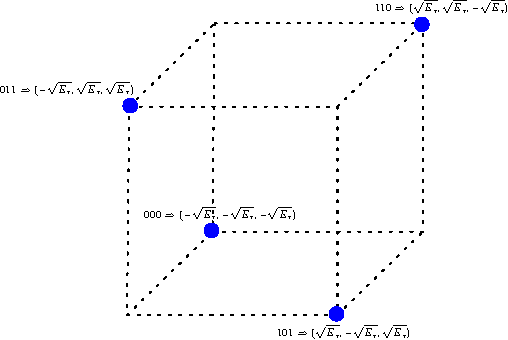
\includegraphics[width=6cm]{./Figuras/DecodificadorBlando}\end{figure*}

La distancia mínima de esta constelación es\footnote{Aunque en este caso es muy sencillo verlo gráficamente, se puede comprobar que en general se cumple que $d_{min} = \sqrt{d_H} \cdot d(a_0,a_1)$, donde $d(a_0,a_1)$ es la distancia entre los símbolos de la constelación binaria ($2\sqrt{E_s}$ en nuestro caso) y $d_H$ la distancia Hamming mínima del código.} $d_{min} = 2 \sqrt{2} \sqrt{E_s}$ y, utilizando la expresión de la cota de la unión simplificada para obtener la probabilidad de error:

\begin{displaymath}
	P_e \leq 3 Q \left ( 2 \sqrt{\frac{E_s}{N_0}} \right )
\end{displaymath}

Igual que hicimos antes podemos calcular el valor de la BER:

\begin{displaymath}
	BER \approx 2Q \left ( 2 \sqrt{\frac{E_s}{N_0}} \right ) = 2Q \left ( \sqrt{\frac{8 E_b}{3 N_0}} \right )
\end{displaymath}

Se puede observar que el valor obtenido será siempre menor al obtenido para el caso de decodificación dura.

A partir de lo visto podemos extraer las siguientes conclusiones:

\begin{itemize}
	\item El uso de un {\bf decodificador duro} nos va a permitir corregir o detectar errores.
	\item El uso de un {\bf decodificador blando} nos va a permitir ``evitar'' los errores, aumentando la distancia mínima del código con respecto a la de la constelación empleada.
\end{itemize}


%%%%%%%%%%%%%%%%%%%%%%%%%%
\section{Códigos cíclicos}\index{Códigos cíclicos}\index{Cíclicos, Códigos}
%%%%%%%%%%%%%%%%%%%%%%%%%%

El principal problema de los códigos convolucionales tal y como los hemos estudiado es que los requisitos hardware para la codificación y decodificación se vuelven prohibitivos en cuanto aumentamos los valores de $n$ y $k$. Los códigos cíclicos son una subclase de códigos bloque que permiten una implementación práctica más sencilla. 

Supongamos que tenemos una palabra código de $n$ bits con la siguiente estructura:

\begin{displaymath}
	\mathbf{c} = (c_0, c_1, \cdots , c_{n-2}, c_{n-1})
\end{displaymath}

Imaginemos ahora que desplazamos circularmente todos los bits de la palabra anterior una posición hacia la derecha. El nuevo vector que obtendríamos sería:

\begin{displaymath}
	\mathbf{c'} = (c_{n-1}, c_0, c_1 \cdots , c_{n-3}, c_{n-2})
\end{displaymath}

Pues bien, decimos que un código lineal es cíclico si cualquier desplazamiento de una palabra código es otra palabra código. Cada una de estas palabras código se puede representar mediante un polinomio binario, que permite realizar la codificación y el cálculo del síndrome de una forma muy eficiente. En nuestro caso, podemos escribir $\mathbf{c}$ como:

\begin{displaymath}
	\mathbf{c} = c_0 + c_1 x + \cdots c_{n-2} x^{n-2} + c_{n-1} x^{n-1}
\end{displaymath}

Donde $x$ es una variable real arbitraria cuyo exponente indica las posiciones de cada uno de los bits en la palabra binaria. 

Si multiplicamos el polinomio $\mathbf{c}$ por $x$,

\begin{displaymath}
	\mathbf{c} x = c_0 x + c_1 x^2 + \cdots c_{n-2} x^{n-1} + c_{n-1} x^{n}
\end{displaymath}

esto se puede reescribir de la siguiente forma, sumando y restando $c_{n-1}$:

\begin{displaymath}
	\mathbf{c} x = c_{n-1} (x^n - 1) + c_{n-1} + c_0 x + c_1 x^2 + \cdots c_{n-2} x^{n-1} 
\end{displaymath}

Es decir, tenemos que:

\begin{displaymath}
	\mathbf{c} x = c_{n-1} (x^n - 1) + \mathbf{c'}
\end{displaymath}

Y aprovechando las propiedades de la suma en módulo 2:

\begin{displaymath}
	\mathbf{c'}= \mathbf{c} x + c_{n-1} (x^n - 1) 
\end{displaymath}

Finalmente, de esta expresión deducimos que el vector $\mathbf{c'}$ se obtiene como el resto de la división de $\mathbf{c} x$ entre $(x^n -1 )$ (operación módulo):

\begin{displaymath}
	\mathbf{c'} = \left ( \mathbf{c} x \right )_{(x^n - 1)}
\end{displaymath}


El polinomio $x^n -1 $ juega un papel muy importante en los códigos cíclicos. De forma más general, se puede comprobar que el desplazamiento cíclico de $i$ posiciones de $\mathbf{c}$ es:

\begin{displaymath}
	\mathbf{c}^{(i)} = (x^i \mathbf{c})_{(x^n -1)}
\end{displaymath}

Aunque en principio pueda parecer que este planteamiento es excesivamente farragoso, la realidad es que de esta forma se pueden sustituir las operaciones matriciales por operaciones polinómicas, mucho más simples de realizar. 

Los códigos cíclicos se caracterizan por tener un {\bf polinomio generador}\index{Polinomio generador} $g(x)$ de grado $r = n-k$ a partir del cual se pueden generar todas las palabras código multiplicándolo por todos los polinomios $b(x)$ de grado máximo $k-1$ que forman las palabras de entrada al codificador. 

Vamos a intentar comprender mejor este procedimiento con un ejemplo. Supongamos que tenemos un código cíclico $n=7$ definido por el siguiente polinomio generador: $g(x) = x^3 + x + 1$. Vamos a obtener todas las posibles palabras código. 

En primer lugar nos fijamos en el orden del polinomio, $r= 3$. De aquí se deduce que $k = n-r = 4$. Para codificar una palabra de entrada cualquiera, por ejemplo \bits{0101}, lo que haremos es, en primer lugar, convertirla a notación polinómica: $b(x) = x^2 + 1$, y a continuación multiplicar este polinomio por el polinomio generador:

\begin{displaymath}
	b(x) \cdot g(x) = (x^2 + 1) \cdot (x^3 + x + 1) = x^5 + x^2 + x +1
\end{displaymath}

Esta expresión, convertida a formato de palabra binaria, sería: \bits{1110010}.

Si repetimos este mismo proceso para todas las demás posibles palabras de entrada de $4$ bits, obtendremos el resultado que se muestra en la siguiente tabla:


\begin{center}
\begin{tabular}{ccl}
\hline
	Mensaje			& Código 			& Polinomio del código \\
	\hline
	\bits{0000}	& \bits{0000000}  & $0\cdot g(x) = 0$ \\
	\bits{0001}	& \bits{1101000}  & $1\cdot g(x) = x^3 + x + 1$ \\
	\bits{0010}	& \bits{0110100}  & $x \cdot g(x) = x^4 + x^2 + x$ \\
	\bits{0011}	& \bits{1011100}  & $(x+1) \cdot g(x) = x^4 + x^3 + x^2 + 1$ \\
	\bits{0100}	& \bits{0011010}  & $x^2 \cdot g(x) = x^5 + x^3 + x^2$ \\
	\bits{0101}	& \bits{1110010}  & $(x^2 +1) \cdot g(x) = x^5 + x^2 + x +1$ \\
	\bits{0110}	& \bits{0101110}  & $(x^2 + x) \cdot g(x) = x^5 + x^4 + x^3 + x$ \\
	\bits{0111}	& \bits{1000110}  & $(x^2+x+1)\cdot g(x) = x^5 + x^4 +1$ \\
	\bits{1000}	& \bits{0001101}  & $(x^3)\cdot g(x) = x^6 + x^4 + x^3$ \\
	\bits{1001}	& \bits{1100101}  & $(x^3+1)\cdot g(x) = x^6 + x^4 + x + 1$ \\
	\bits{1010}	& \bits{0111001}  & $(x^3+x)\cdot g(x) = x^6 + x^3 + x^2 + x$ \\
	\bits{1011}	& \bits{1010001}  & $(x^3 + x +1)\cdot g(x) = x^6 + x^2 + 1$ \\
	\bits{1100}	& \bits{0010111}  & $(x^3+x^2)\cdot g(x) = x^6+x^5+x^4 +x^2$ \\
	\bits{1101}	& \bits{1111111}  & $(x^3+x^2+1)\cdot g(x) = x^6+x^5+x^4+x^3+x^2+x+1$ \\
	\bits{1110}	& \bits{0100011}  & $(x^3+x^2+x)\cdot g(x) = x^6+x^5+x$ \\
	\bits{1111}	& \bits{1001011}  & $(x^3+x^2+x+1)\cdot g(x) = x^6+x^5+x^3+1$ \\ 
\hline
\end{tabular}
\end{center}

Como se podrá observar, el código que hemos construido no es sistemático, esto es, los bits de la entrada no forman parte de la salida. Existe un procedimiento para obtener una versión sistemática de un código cíclico que, aunque algo más complicado que el anterior, resulta muy sencillo de entender con un ejemplo. 

El procedimiento se basa en crear la palabra código resultante, $c(x)$, a partir del polinomio generador $g(x)$ de la forma:

\begin{displaymath}
	c(x) = b(x) x^{n-k} + d(x)
\end{displaymath}

donde $d(x)$ se obtiene mediante como el resto de dividir $b(x) x^{n-k}$ por $g(x)$.

En nuestro ejemplo anterior, donde $g(x)=x^3+x+1$, $n=7$ y se deseaba codificar la palabra \bits{1001}, haremos lo siguiente:

\begin{enumerate}
	\item Dividimos $b(x)x^3$ entre $g(x)$, obteniéndose que el resto es $d(x) = x^2+x$.
	\item Construimos la palabra código como $c(x) = b(x) x^{n-k} + d(x)$. Así:
	\begin{displaymath}
		c(x) = x^6+x^3+x^2+x \Rightarrow \mathbf{c} = [\bits{0111001}]
	\end{displaymath}
\end{enumerate} 



En cuanto a la decodificación, debemos obtener el polinomio de comprobación de paridad, $h(x)$, que cumple que:

\begin{displaymath}
	\left ( g(x) h(x) \right )_{(x^n-1)} = 0
\end{displaymath}

El síndrome será ahora un polinomio de grado $n-k-1$ que se obtiene a partir del polinomio recibido $r(x)$:

\begin{displaymath}
	s(x) = \left ( r(x) h(x) \right )_{(x^n - 1)}
\end{displaymath}

Hemos visto cómo realizar la codificación y decodificación de los códigos binarios cíclicos, pero no hemos visto cómo diseñarlos para cumplir algún determinado requisito de detección y corrección de errores. Para ello es necesario recurrir a la estructura algebraica de los cuerpos de Galois basados en polinomios, y en este sentido se han propuesto distintos algoritmos entre los que los más conocidos son el BCH (propuesto por Bose, Chaudhuri y Hocquenghem) o los Reed-Solomon. 

Vamos a ver, de forma muy simplificada, la forma de diseñar el polinomio generador de un código cíclico BCH de longitud $n$ y con capacidad para corregir $t$ errores. 

En concreto vamos a verlo para el caso particular de $n=15$ y $t=2$.

El proceso consta de los siguientes pasos:

\begin{enumerate}
	\item {\bf Calcular el valor de $m$}
	
	En este paso se trata de encontrar un $m$ tal que $((2^m-1))_n = 0$.
	En nuestro caso es sencillo ver que si $m=4$, $2^m-1 = 15$ y $((15))_{15} = 0$.	
	
	\item {\bf Encontrar un polinomio primitivo de grado $m$}
	
	Un polinomio primitivo es aquel polinomio que no es posible factorizar en un producto de polinomios de menor grado y que cumple que el menor entero $n$ para el cual divide a $x^n -1$ es $n=2^m -1$.
	
	En este cuadro se muestran los polinomios primitivos de grado 2 a 0:
	
\begin{center}
\begin{tabular}{l}
\hline
	$p_{2}(x) = x^2+x+1$ \\
	$p_{3}(x) = x^3+x+1$ \\
	$p_{4}(x) = x^4+x+1$ \\
	$p_{5}(x) = x^5+x^2+1$ \\
	$p_{6}(x) = x^6+x+1$ \\
	$p_{7}(x) = x^7+x+1$ \\
	$p_{8}(x) = x^8+x^4+x^3+x^2+1$ \\
	$p_{9}(x) = x^9+x^4+1$ \\
	$p_{10}(x) = x^{10}+x^3+1$ \\
\hline
\end{tabular}
\end{center}
	
	Siguiendo con nuestro ejemplo, y dado que habíamos visto que $m=4$, tomaremos el polinomio $p_4(x)=x^4+x+1$.
	
	\item {\bf Generar los elementos del cuerpo de Galois}
	 
	 Como decíamos antes, la estructura algebraica de los códigos sistemáticos se sustenta sobre la base de los cuerpos de Galois. En este caso tenemos que generar los elementos de un cuerpo de Galois $GF(2^m)$. La forma más sencilla de hacer esto es calcular todas las posibles raíces de $x^n -1$, de forma que:
	 
	 \begin{displaymath}
	 	x^n -1 = (x-\alpha^0)\cdot (x-\alpha^1) \cdot (x-\alpha^2) \cdots (x-\alpha^{2^m-2})
	 \end{displaymath}
	 
	 La forma de hacerlo es partiendo de una raíz $\alpha^0 = 1$ y generando las siguientes, hasta $\alpha^{2^m-2}$ de la siguiente forma:
	 
	 \begin{displaymath}
	 	\alpha^{i} = ((\alpha^{i-1}))_{p_m(x)}
	 \end{displaymath}
	 
	 En nuestro caso:
	 
\begin{center}
\begin{tabular}{l}
\hline
	$\alpha^0 = 1$ \\
	$\alpha^1 = x$ \\
	$\alpha^2 = x^2$ \\
	$\alpha^3 = x^3$ \\
	$\alpha^4 = ((x^4))_{x^4+x+1} = x+1$ \\
	$\alpha^5 = x^2+x$ \\
	$\alpha^6 = x^3+x^2$ \\
	$\alpha^7 = ((x^4+x^3))_{x^4+x+1} = x^3+x+1$ \\
	$\alpha^8 = x^2+1$ \\
	$\alpha^9 = x^3+x$ \\
	$\alpha^{10} = x^2+x+1$ \\
	$\alpha^{11} = x^3+x^2+x$ \\
	$\alpha^{12} = x^3+x^2+x+1$ \\
	$\alpha^{13} = x^3+x^2+1$ \\
	$\alpha^{14} = x^3+1$ \\
\hline
\end{tabular}
\end{center}
	 
	A partir de aquí es fácil comprobar que $\alpha^{15} = \alpha^0$, y en general que $\alpha^{i} = \alpha^{((i))_{2^m-1}}$.
	
	
	\item {\bf Construir las clases conjugadas y los polinomios minimales}
	
	Para crear la primera clase conjugada tomaremos la raíz $\alpha$ y contruimos la secuencia de cuadrados consecutivos $\alpha, \alpha^2, \alpha^4, \alpha^8, etc.$ y crearemos un polinomio que contenga todas estas raíces: $(x-\alpha)(x-\alpha^2)(x-\alpha^4)\cdots$
	
	Haremos lo mismo para el resto de las raíces, y obtendremos:
	
\begin{center}
\begin{tabular}{ll}
\hline
	Clases conjugadas							& Polinomios minimales \\
	\hline
	$\{\alpha^0\}$								& $m_0(x) = x-1$ \\
	$\{\alpha,\alpha^2,\alpha^4, \alpha^8\}$ 	& $m_1(x) = x_4+x+1$ \\
	$\{\alpha^3,\alpha^6,\alpha^{12}, \alpha^{((24))_{15}} =\alpha^{9}\}$ 	& $m_3(x) = x^4+x^3+x^2+x+1$ \\
	$\{\alpha^5,\alpha^{10}\}$ 	& $m_5(x) = x^2+x+1$ \\
	$\{\alpha^7,\alpha^{14}, \alpha^{((28))_{15}} =\alpha^{13}, \alpha^{((56))_{15}} =\alpha^{11}\}$ 	& $m_7(x) = x^4+x^3+1$ \\
\hline
\end{tabular}
\end{center}
	
	\item {\bf Construir el polinomio generador}
	
	El último paso consiste en construir el polinomio generador de menor grado posible que contenga $2t$ raíces consecutivas de $x^n-1$ partir de sus polinomios minimales. 
	
	En nuestro ejemplo podemos ver que ninguna de las clases conjugadas tiene 4 raíces consecutivas, pero si combinamos, por ejemplo, la segunda con la tercera, obtenemos el conjunto $\{\alpha,\alpha^2,\alpha^3,\alpha^4, \alpha^6, \alpha^8, \alpha^9, \alpha^{12}\}$ donde sí que hay cuatro raíces consecutivas: $\alpha,\alpha^2,\alpha^3,\alpha^4$.
	
	Así, finalmente el polinomio generador será:
	
	\begin{displaymath}
		g(x) = m_1(x)\cdot m_3(x) = x^8+x^7+x^6+x4+1
	\end{displaymath}
	
	 
\end{enumerate}



%%%%%%%%%%%%%%%%%%%%%%%%%%%%%%%%%
\section{Códigos convolucionales}\index{Código convolucional}\index{Convolucional, Código}
%%%%%%%%%%%%%%%%%%%%%%%%%%%%%%%%%

Los códigos convolucionales se diferencian de los códigos bloque lineales que hemos estado viendo hasta ahora en que tienen memoria, y su salida se calcula mediante a una operación que recuerda a una convolución. 

Para entender mejor su funcionamiento vamos a utilizar el ejemplo mostrado en la Figura \ref{fig:CodificadorConvolucional}.


%El bloque básico de un codificador convolucional es el registro de desplazamiento, mostrado en la Figura \ref{fig:RegistroDesplazamiento}. Cada una de las ganancias $g_i$ representa un cortocircuito o un circuito abierto, y los bits del registro se combinan mediante suma módulo 2 para obtener los bits codificados a la salida:
%
%\begin{figure*}
%	\label{fig:RegistroDesplazamiento}
%	\centering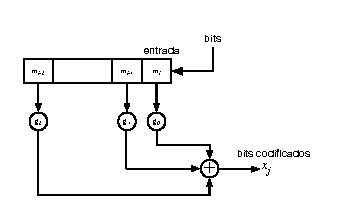
\includegraphics[width=10cm]{RegistroDesplazamiento}
%		\caption{Esquema de un registro de desplazamiento utilizado en los códigos convolucionales.}	
%\end{figure*}
%
%\begin{displaymath}
%	x_j = m_{j-L} g_L \oplus \cdots m_{j-1}g_1 \oplus m_j g_0 
%\end{displaymath}
%
%Si nos fijamos, vemos que el bit $x_j$ depende no sólo del bit actual, $m_j$ sino también de los $L$ bits del mensaje anteriores. 
%
%Con el registro de desplazamiento tal cual lo hemos representado, estamos obteniendo bits a la salida al mismo ritmo que entran los bits a la entrada. No se trata, por tanto, de un codificador, ya que no se introducen bits extra que puedan servir para el control de errores. 
%
%Para conseguirlo, lo que haremos será añadir más sumadores módulo 2 a la salida, tal y como se muestra por ejemplo en la Figura \ref{fig:CodificadorConvolucional}.

Como se puede observar, el codificador consta de un registro de desplazamiento con dos retardos. Cada nuevo bit introducido a la entrada del codificador, $m_j$, se combina con los dos bits anteriores almacenados en el registro, $m_{j-1}$ y $m_{j-2}$ para formar dos bits codificados que constituirán la salida del codificador, $x'_j$ y $x''_j$. 

\begin{figure*}[h!]
	\centering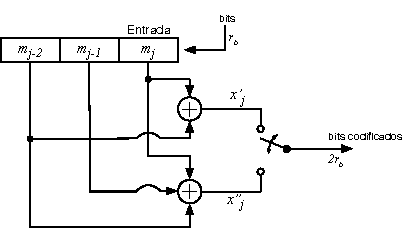
\includegraphics[width=10cm]{./Figuras/CodificadorConvolucional}
	\caption{Esquema de un codificador convolucional con $n=2$, $k=1$ y $L=2$.}	
	\label{fig:CodificadorConvolucional}
\end{figure*}


A partir de la figura podemos ver que los bits que se generan a la salida responden a la siguiente expresión:

\begin{displaymath}
	\begin{array}{l}
		x'_j = m_j \oplus m_{j-2} \\
		x''_j = m_j \oplus m_{j-1} \oplus m_{j-2} \\
	\end{array}
\end{displaymath}


Estos bits finalmente se intercalan entre sí para obtener la trama binaria de salida:

\begin{displaymath}
	\mathbf{x} = (x'_1 \,\, x''_1 \,\, x'_2 \,\, x''_2 \,\, x'_3 \,\, x''_3 \,\, \cdots )
\end{displaymath}

Podemos ver que se trata de un codificador con una tasa de codificación $R_c = 1/2$, ya que por cada bit a la entrada ($k=1$) se obtienen dos bits a la salida ($n=2$). Además, al número de retardos que introduce el sistema, en nuestro caso $L=2$ se le denomina {\bf memoria} del codificador. 

El ejemplo mostrado, por tanto, se corresponde con un código convolucional $(n,k,L)$ con $n=2$, $k=1$ y $L=2$.

Si suponemos un estado inicial en el que todos los registros estén a cero ($m_{j-1} = m_{j-2} = \mathtt{0}$) podemos a partir de ahí intentar representar todos los posibles estados del codificador en función de las posibles entradas y obtener así una representación en forma de árbol como la mostrada en la Figura \ref{fig:ArbolCodigoConvolucional}\index{Diagrama de árbol}. 

\begin{figure*}
	\centering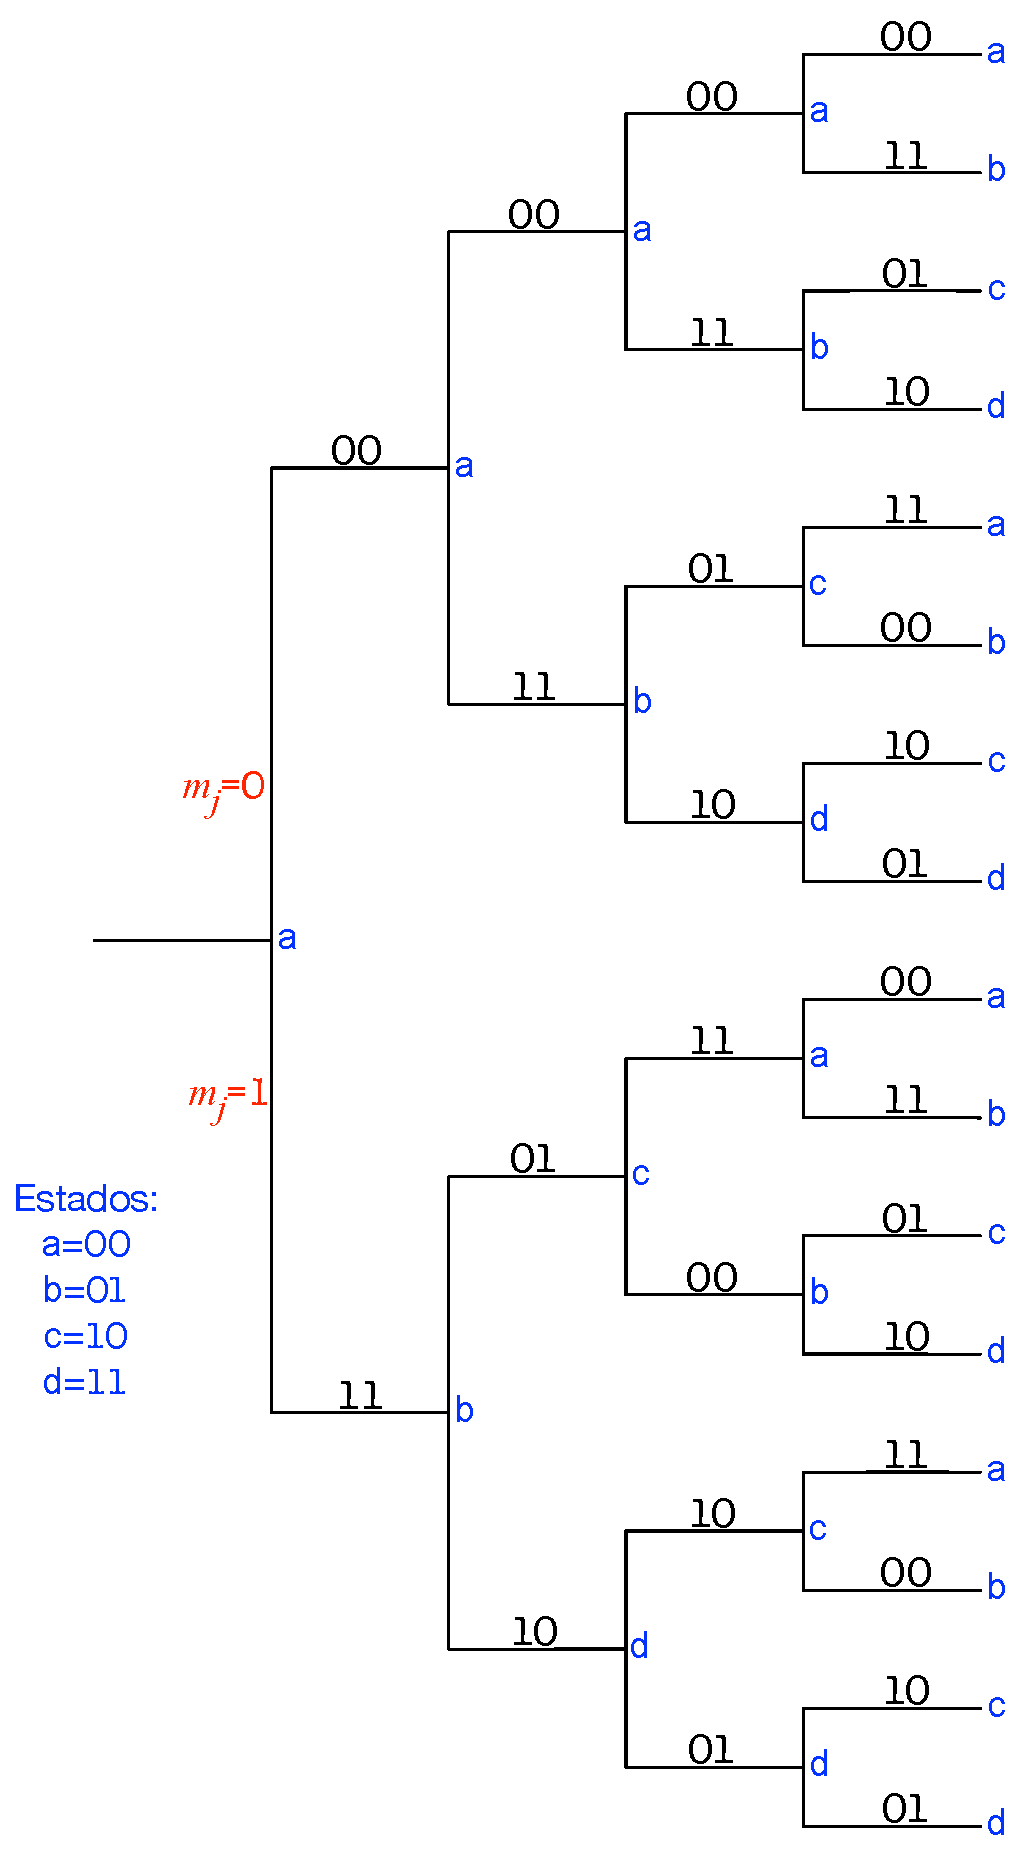
\includegraphics[width=5cm]{./Figuras/ArbolCodigoConvolucional}
		\caption{Diagrama de árbol para el código convolucional $(2,1,2)$ del ejemplo.}	
		\label{fig:ArbolCodigoConvolucional}
\end{figure*}

El codificador podrá estar en cuatro estados distintos, marcados por los valores de los bits almacenados en el registro: $(m_{j-2}, m_{j-1})$. Por claridad, denominamos a los estados por letras: $a=\mathtt{00}$, $b=\mathtt{01}$, $c=\mathtt{10}$ y $d=\mathtt{11}$. Si, por ejemplo, el codificador se encuentra inicialmente en el estado $a$ (\bits{00}) y el bit a la entrada es $m_j = 1$, el nuevo estado del codificador será el $b$ (\bits{01}). En la Figura \ref{fig:ExplicacionEstado} se muestra este caso y la evolución si la secuencia a la entrada es \bits{1101}.

\begin{figure*}
	\centering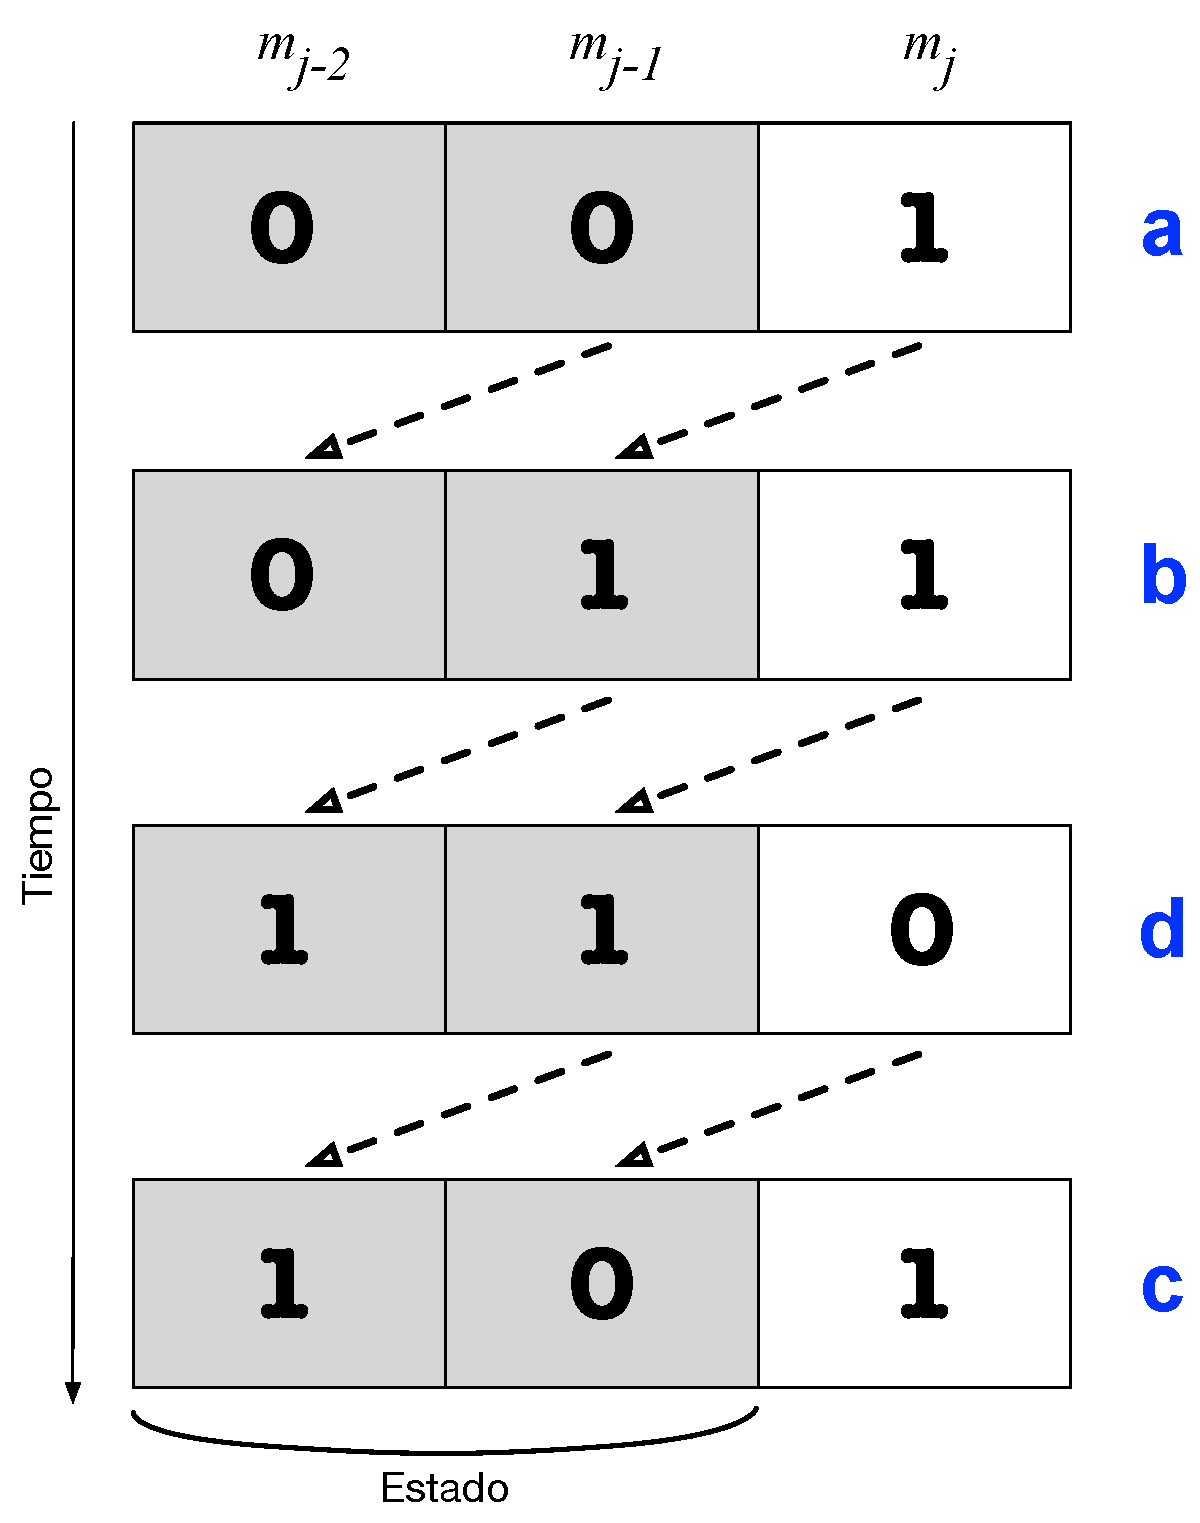
\includegraphics[width=5cm]{./Figuras/ExplicacionEstado}
		\caption{Evolución de los estados en un codificador convolucional.}	
	\label{fig:ExplicacionEstado}
\end{figure*}

Además de mostrar las transiciones entre estados del codificador, el diagrama de árbol también nos muestra la salida del codificador cuando se pasa de un estado a otro. 

Así, por ejemplo, si partimos como antes del estado \bits{00} y el bit de entrada al codificador es $m_j = \mathtt{0}$, entonces la salida será:

\begin{displaymath}
\begin{array}{l}
	x'_j = m_j \oplus m_{j-2} = \mathtt{0} \oplus \mathtt{0} = \mathtt{0}\\
	x''_j = m_j \oplus m_{j-1} \oplus m_{j-2} = \mathtt{0} \oplus \mathtt{0} \oplus \mathtt{0} = \mathtt{0}
\end{array}
\end{displaymath}


La salida será por tanto $(x'_j x''_j) = (\mathtt{0\, 0})$. Por otra parte, si la entrada fuese $m_j = \mathtt{1}$, entonces:

\begin{displaymath}
\begin{array}{l}
	x'_j = m_j \oplus m_{j-2} = \mathtt{1} \oplus \mathtt{0} = \mathtt{1} \\
	x''_j = m_j \oplus m_{j-1} \oplus m_{j-2} = \mathtt{1} \oplus \mathtt{0} \oplus \mathtt{0} = \mathtt{1}
\end{array}
\end{displaymath}


En este caso la salida es $(x'_j x''_j) = (\mathtt{1\, 1})$. Es decir, del estado $a$ se puede pasar al estado $a$ de nuevo si la entrada es \bits{0} (produciendo una salida $\mathtt{0 \, 0}$) o bien al estado $b$, si la entrada es \bits{1} (siendo en este caso la salida $\mathtt{1 \, 1}$).

Esto es lo que podemos ver representado en el árbol de codificador. Si ahora suponemos que estamos en el estado $d = \mathtt{11}$ y que la entrada es $\mathtt{0}$, entonces ahora tendremos:

\begin{displaymath}
\begin{array}{l}
	x'_j = m_j \oplus m_{j-2} = \mathtt{0} \oplus \mathtt{1} = \mathtt{1}\\
	x''_j = m_j \oplus m_{j-1} \oplus m_{j-2} = \mathtt{0} \oplus \mathtt{1} \oplus \mathtt{1} = \mathtt{0}
\end{array}
\end{displaymath}


Habremos pasado del estado $d=\mathtt{1\, 1}$ al $c=\mathtt{1\, 0}$ produciendo una salida igual a $\mathtt{1 \, 0}$. Siguiendo este mismo proceso podemos ir construyendo todas las ramas del árbol, y si nos damos cuenta a partir de un determinado momento se va a ir repitiendo, dado que el codificador sólo cuenta con dos retardos, y por tanto la salida nunca va a depender de más de 2 bits anteriores al actual.


Una forma más compacta de representar todas las posibles transiciones entre estados en un codificador convolucional es mediante un diagrama de rejilla\index{Diagrama de rejilla} o un diagrama de estados\index{Diagrama de estados}, tal y como se muestra en la figura \ref{fig:RejillayEstadosCodigoConvolucional}. 


\begin{figure*}
	\centering
	\subfigure{\label{fig:RejillaCodigoConvolucional}\centering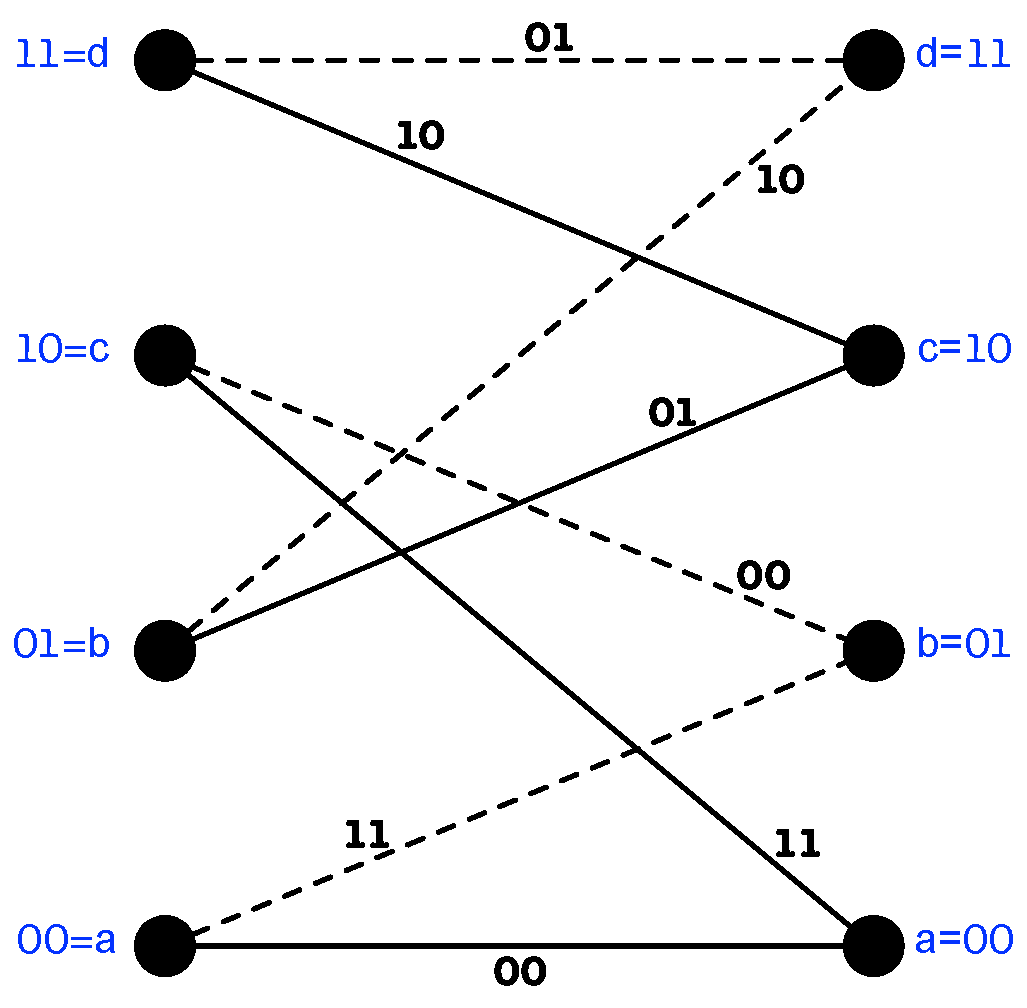
\includegraphics[width=6cm]{./Figuras/RejillaCodigoConvolucional2}}
	\subfigure{\label{fig:EstadosCodigoConvolucional}\centering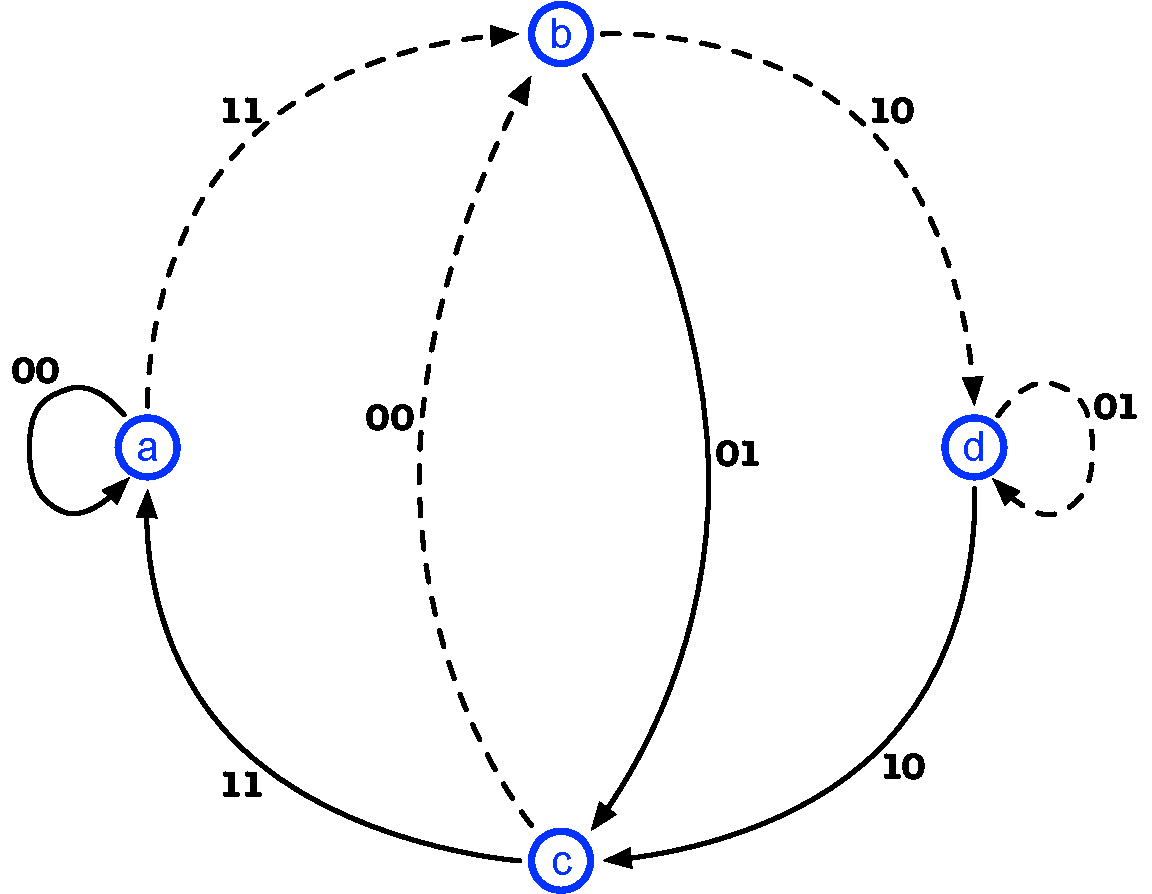
\includegraphics[width=6cm]{./Figuras/EstadosCodigoConvolucional}}
		\caption{Diagrama de rejilla \subref{fig:RejillaCodigoConvolucional} y diagrama de estados \subref{fig:EstadosCodigoConvolucional} para el código convolucional $(2,1,2)$ del ejemplo.}	
		\label{fig:RejillayEstadosCodigoConvolucional}
\end{figure*}

Ambas representaciones muestran esencialmente lo mismo: las distintas transiciones posibles entre los estados del codificador y los bits que se obtienen a la salida para cada una de estas transiciones.

Una última forma de analizar este tipo de códigos es haciendo uso de polinomios en $D$ ($D$ representa un retardo unidad, equivalente a la $z^{-1}$ de la Transformada Z). Así, utilizando esta notación, nuestro codificador de ejemplo se podría representar mediante los siguientes polinomios generadores\index{Polinomio generador}:

\begin{displaymath}
\begin{array}{l}
	G_1(D) = 1 + D^2\\
	G_2(D) = 1 + D^1 + D^2
\end{array}
\end{displaymath}


Esta representación nos permite obtener de forma muy sencilla la salida del codificador a cualquier secuencia binaria de entrada. Si, por ejemplo, tuviésemos a la entrada la secuencia $\mathtt{110111001000}$, que puede escribirse de forma polinomial como $1 + D + D^3 + D^4 + D^5 + D^8$, la salida vendrá dada por:

\begin{displaymath}
	\begin{array}{ll}
	X'_j(D) & = M(D) G_1(D) = (1 + D + D^3 + D^4 + D^5 + D^8) (1 + D^2) = \\
			& = 1 + D + D^2 + D^4 + D^6 + D^7 + D^8 + D^{10} = \mathtt{11101011101}
	\end{array}
\end{displaymath}

\begin{displaymath}
	\begin{array}{ll}
	X''_j(D) & = M(D) G_2(D) = (1 + D + D^3 + D^4 + D^5 + D^8) (1 + D^1 + D^2) = \\
			& = 1 + D^5 + D^7 + D^8 + D^9 + D^{10} = \mathtt{10000101111}
	\end{array}
\end{displaymath}

Finalmente, la salida se obtiene intercalando los bits anteriores:

\begin{displaymath}
	x_j = \mathtt{11\, 10\, 10\, 00\, 10\, 01\, 10\, 11\, 11\, 01\, 11}
\end{displaymath}


%%%%%%%%%%%%%%%%%%%%%%%%%%%%%%%%%%%%%%%%%%%%%%%%%%
\subsection{Decodificación. Algoritmo de Viterbi}\index{Viterbi, Algoritmo de}
%%%%%%%%%%%%%%%%%%%%%%%%%%%%%%%%%%%%%%%%%%%%%%%%%%

Existen varias formas de decodificar una secuencia binaria obtenida con un codificador convolucional. Nosotros no obstante nos vamos a centrar en estudiar el algoritmo de Viterbi, que permite implementar un receptor de máxima verosimilitud aunque a costa de un gran consumo de memoria por parte del decodificador. 

Vamos a seguir con nuestro codificador de ejemplo, que recordamos venía dado por las siguientes expresiones:

\begin{displaymath}
	\begin{array}{l}
		x'_j = m_j \oplus m_{j-2} \\
		x''_j = m_j \oplus m_{j-1} \oplus m_{j-2} \\
	\end{array}
\end{displaymath}

Vamos a suponer que partimos del estado inicial $a=\mathtt{00}$ y que también terminamos en ese mismo estado (para ello basta con añadir dos ceros al final de la secuencia recibida). Supongamos también que la secuencia transmitida es $\mathtt{11010100}$ (ya hemos incluido los dos ceros al final para asegurar que el último estado sea el \bits{00}. La salida del codificador para esta secuencia de entrada es: $\mathtt{11\,10\,10\, 00\, 01 \, 00 \, 01 \, 11}$. 

Supondremos por último que el canal es ideal, y que por tanto la secuencia recibida es exactamente igual a la transmitida, sin errores. 

En la Figura \ref{fig:Viterbi_1} se muestran las dos primeras iteraciones del algoritmo. La secuencia de entrada se muestra en la parte inferior, y en el interior de cada nodo se muestra la distancia Hamming acumulada hasta ese punto. Partiendo del estado \bits{00} existen dos opciones: 

\begin{itemize}
	\item Ir al estado $b = \mathtt{01}$, con lo que la salida del codificador sería \bits{11}, tal y como indicamos junto a la flecha de la transición. En este caso la distancia Hamming entre esta salida (\bits{11}) y la entrada al codificador (\bits{11}) será cero. 
	\item Continuar en el estado $a = \mathtt{00}$, siendo en este caso la salida del codificador \bits{00}. La distancia Hamming entre la salida (\bits{00}) y la entrada (\bits{11}) es de dos. 
\end{itemize}

En la segunda iteración repetimos el proceso, partiendo de los dos nodos que tenemos ahora ``activos''. Tenemos cuatro opciones:

\begin{itemize}
	\item Pasar del estado $a$ al $a$, sumando uno a la distancia Hamming acumulada, con lo que ahora sería de tres. 
	\item Pasar del estado $a$ al $b$, obteniendo una distancia acumulada de tres.
	\item Pasar del estado $b$ al $c$, que supone añadir dos a la distancia acumulada hasta entonces.
	\item Pasar del estado $b$ al $d$, que suma cero a la distancia acumulada, manteniéndose ésta en este valor, por tanto. 
\end{itemize}


\begin{figure*}
		\centering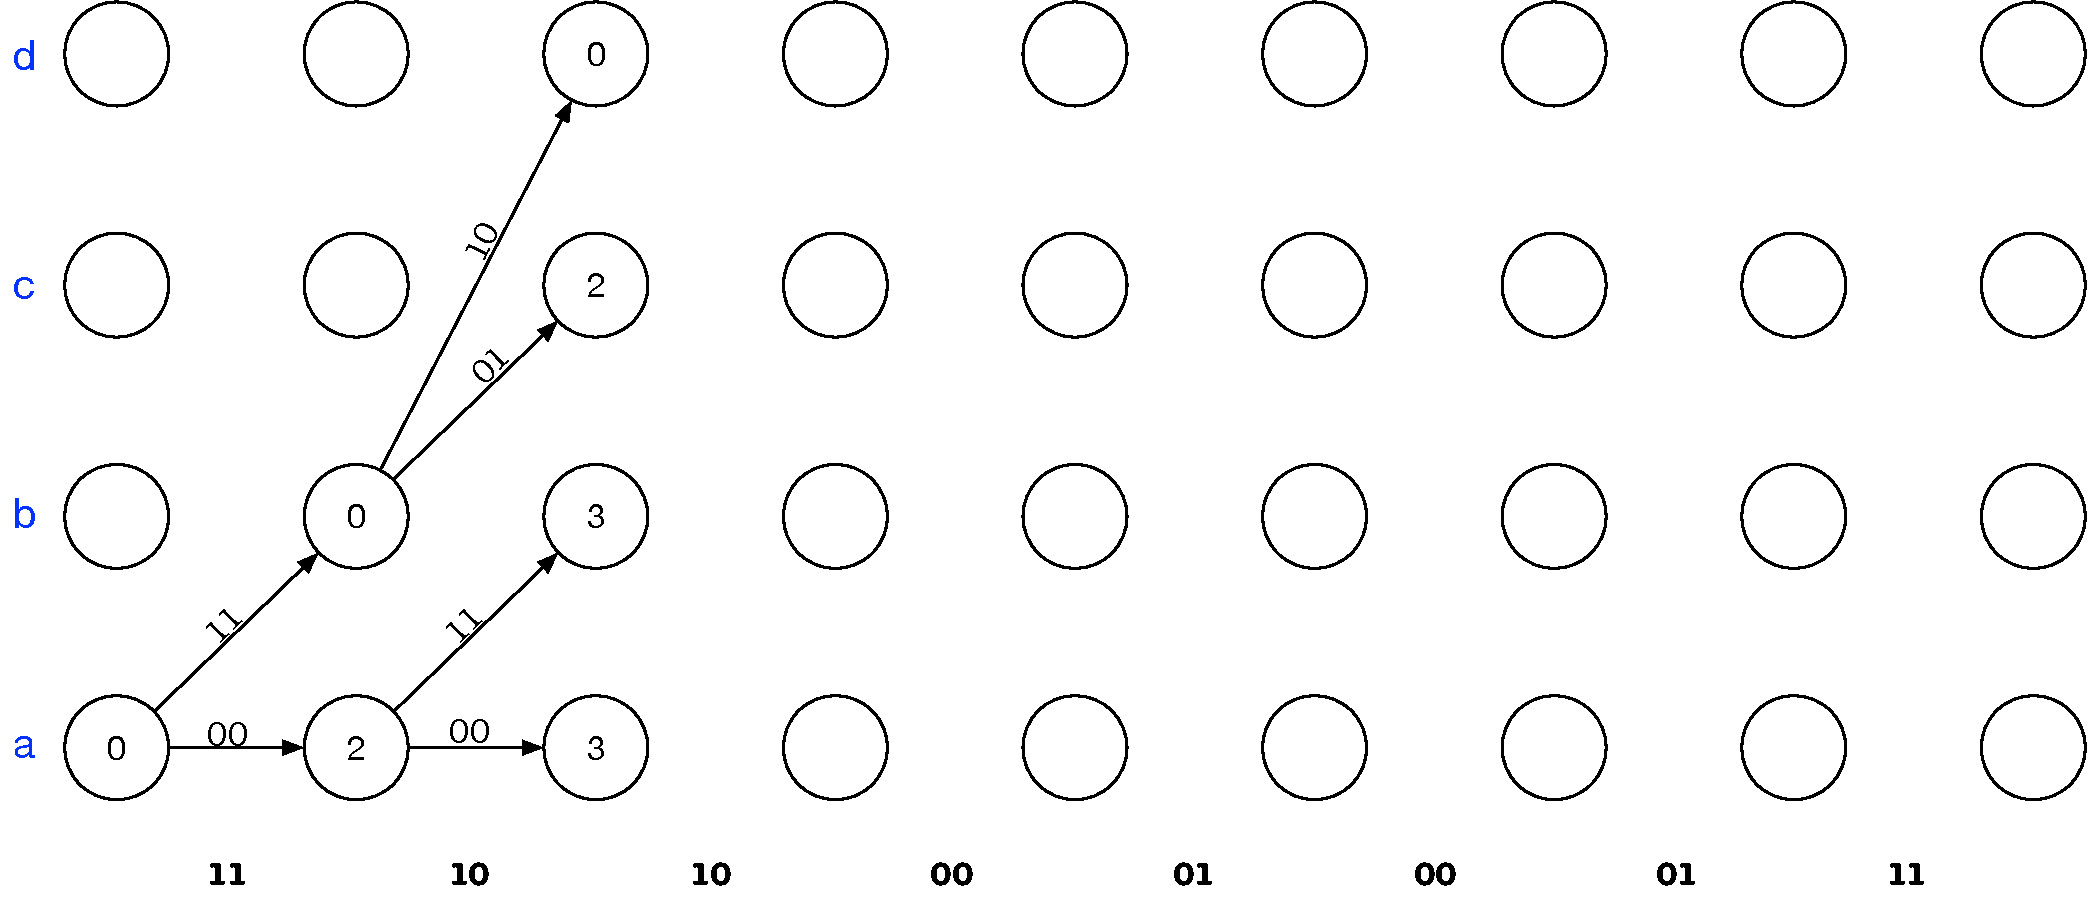
\includegraphics[width=10cm]{./Figuras/Viterbi_1}
		\caption{Primeras dos iteraciones del algoritmo de Viterbi.}	
		\label{fig:Viterbi_1}
	\end{figure*}

Llegamos ahora a la tercera iteración, mostrada en la Figura \ref{fig:Viterbi_2}. El proceso es idéntico al que hemos seguido hasta ahora, aunque ahora nos encontramos con que a cada estado podemos llegar desde dos estados distintos. Por ejemplo, al estado $d$ se puede llegar desde el propio estado $d$, añadiendo dos a la distancia acumulada, que totalizaría dos, o bien desde el estado $b$, siendo en este caso la distancia acumulada igual a tres (tres del estado anterior más cero debido a esta transición). Lo que haremos en este caso es descartar aquel camino con una mayor distancia acumulada (el que viene del nodo $b$, y que está marcado con línea de puntos en la figura), dejando únicamente ``vivo'' el camino con menor distancia Hamming acumulada. 


\begin{figure*}
	\centering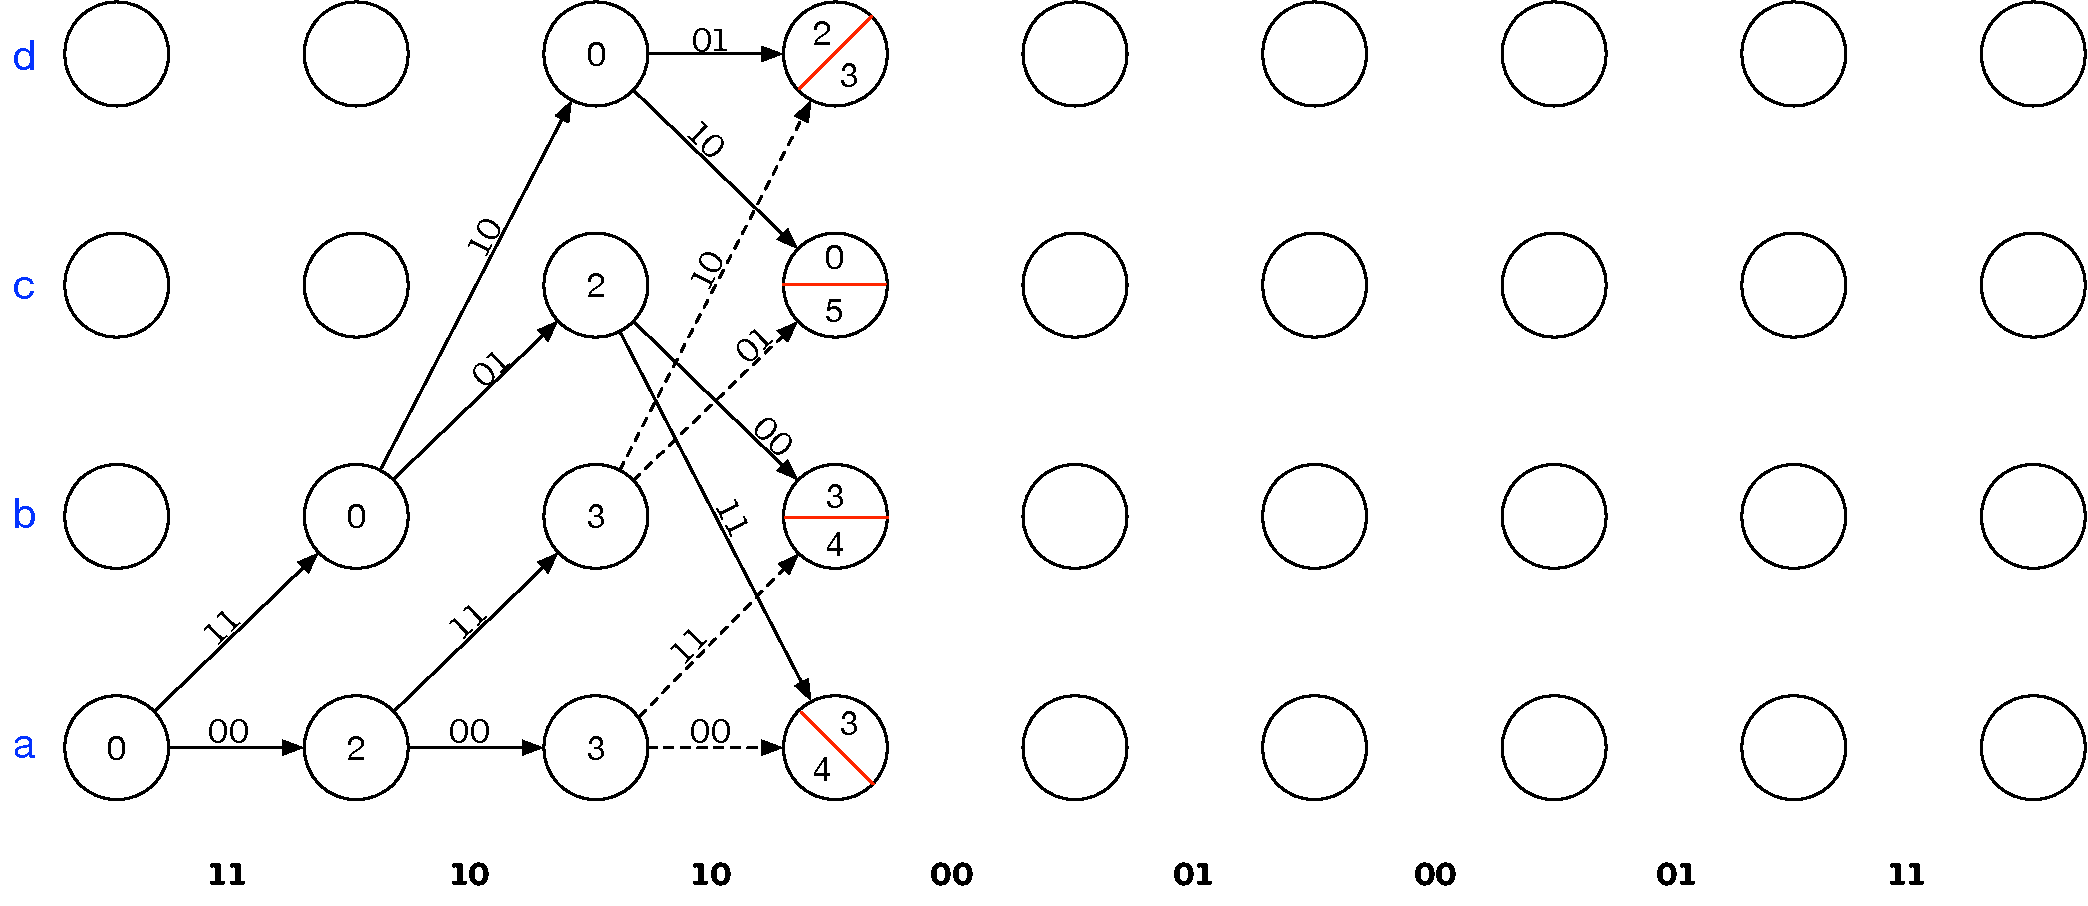
\includegraphics[width=10cm]{./Figuras/Viterbi_2}
		\caption{Tercera iteración del algoritmo de Viterbi.}	
		\label{fig:Viterbi_2}
\end{figure*}

En la figura \ref{fig:Viterbi_3} se muestra cómo quedaría el diagrama una vez que hayamos eliminado los caminos con mayor distancia acumulada en cada uno de los nodos. 

\begin{figure*}
	\centering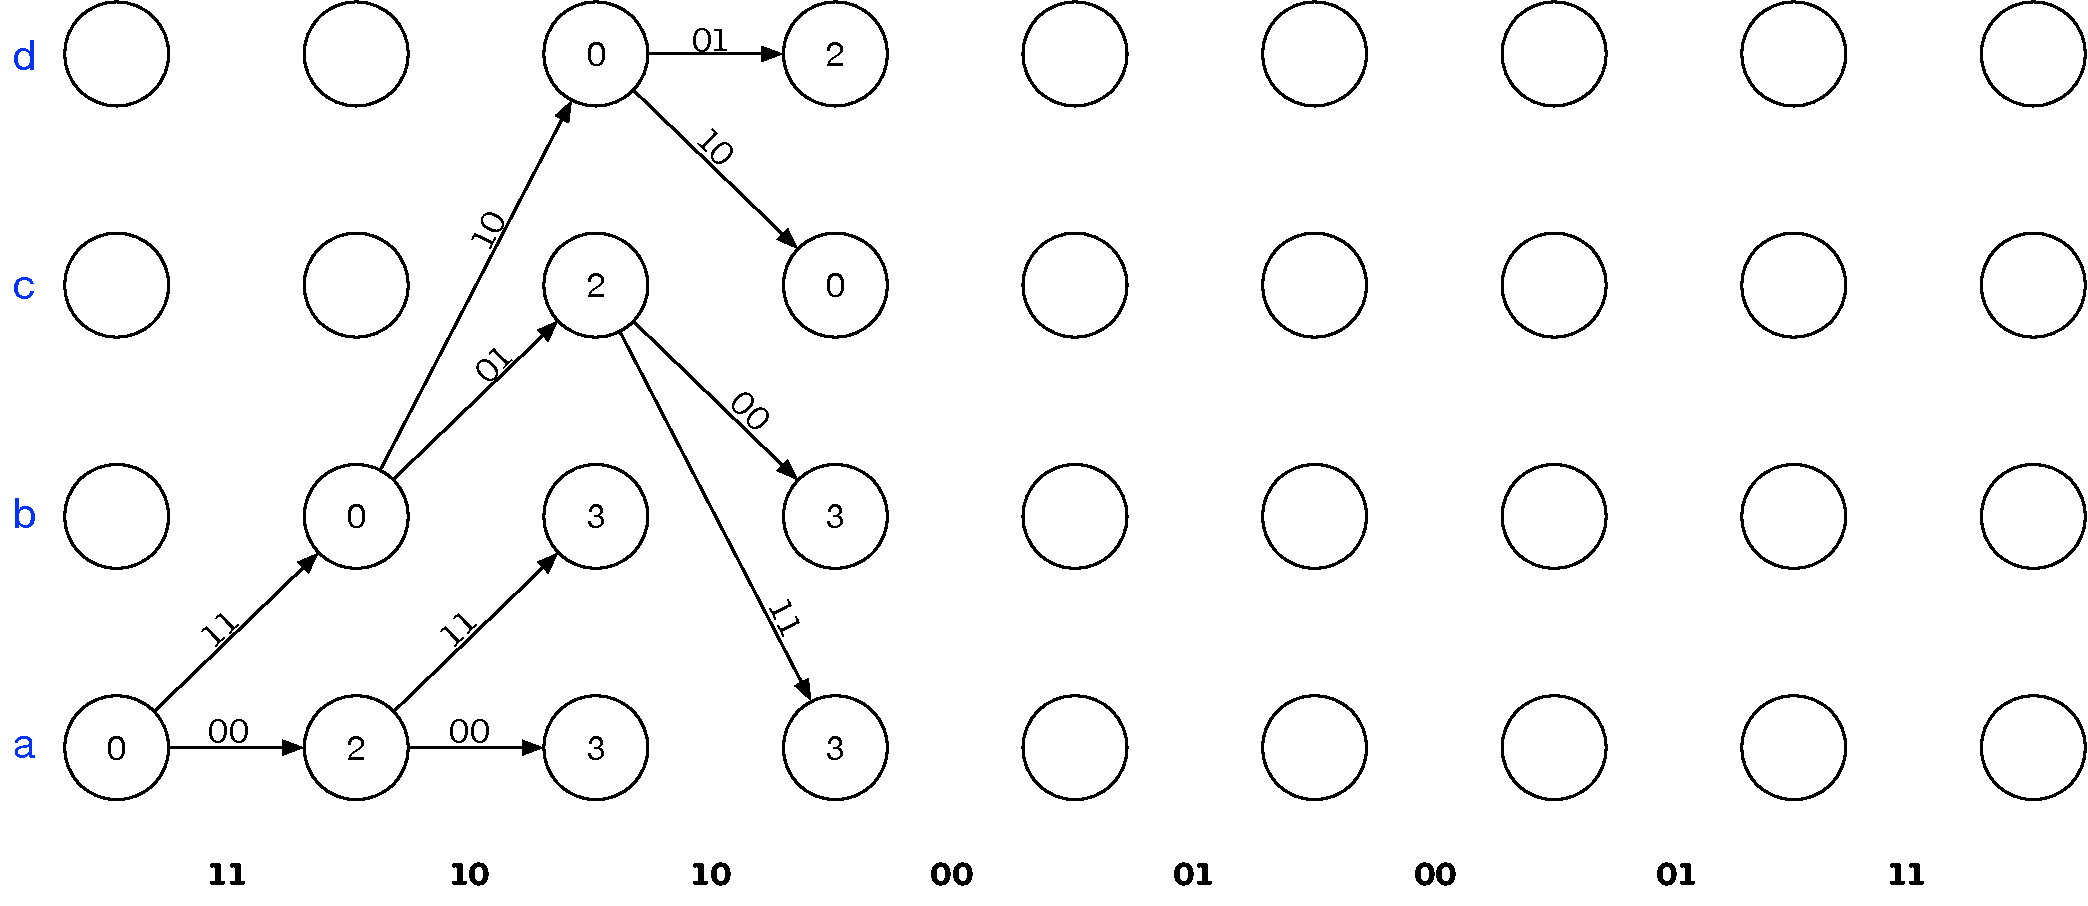
\includegraphics[width=10cm]{./Figuras/Viterbi_3}
		\caption{tercera iteración del algoritmo de Viterbi, tras eliminar los caminos con mayor distancia Hamming acumulada.}	
		\label{fig:Viterbi_3}
\end{figure*}


En la Figura \ref{fig:Viterbi_4} se muestra la siguiente iteración del algoritmo, con los caminos con mayor distancia acumulada marcados con línea discontinua. 

\begin{figure*}
	\centering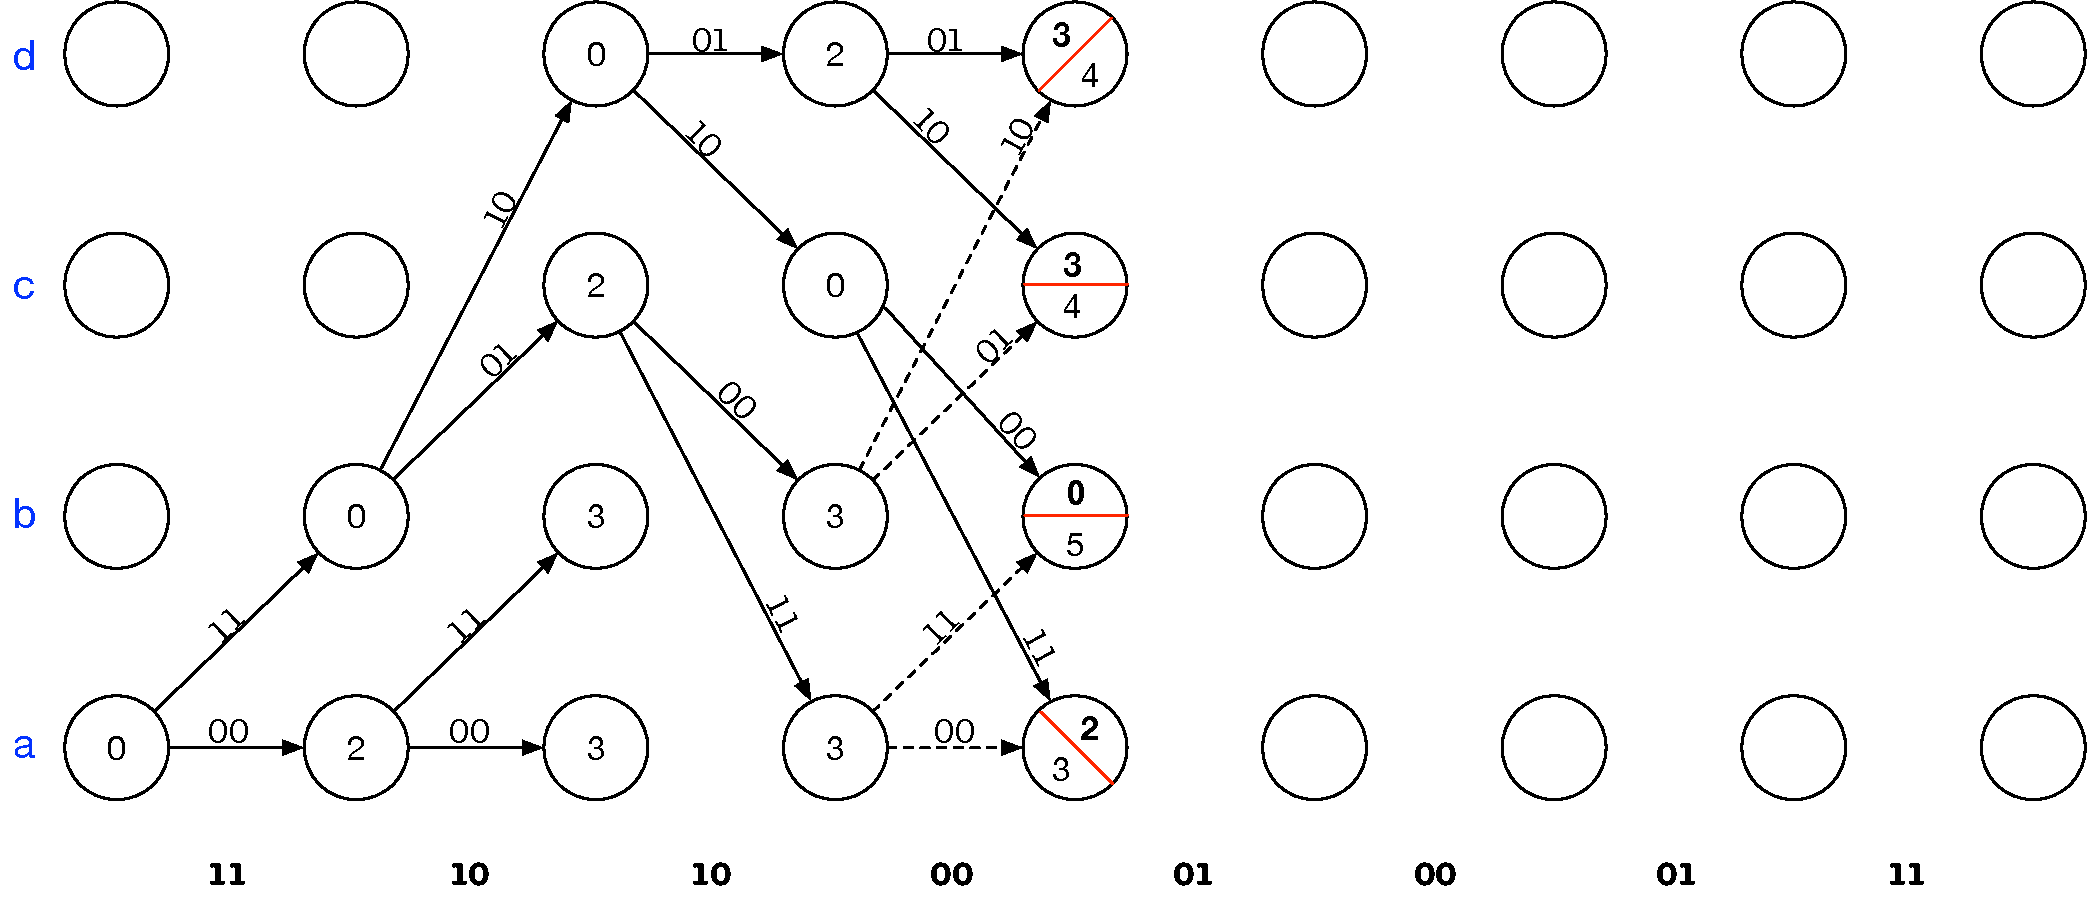
\includegraphics[width=10cm]{./Figuras/Viterbi_4}
		\caption{Cuarta iteración del algoritmo de Viterbi.}	
		\label{fig:Viterbi_4}
\end{figure*}

Por último, en la figura \ref{fig:Viterbi_5} se muestra el estado final del algoritmo, una vez que hemos llegado al último estado. El camino con menor distancia Hamming acumulada se ha destacado en línea más gruesa. Podemos comprobar que la salida del sistema para este camino coincide de forma exacta con la entrada, algo que no nos debería sorprender, pues hemos supuesto que no ha habido ningún error en la transmisión. 

\begin{figure*}
	\centering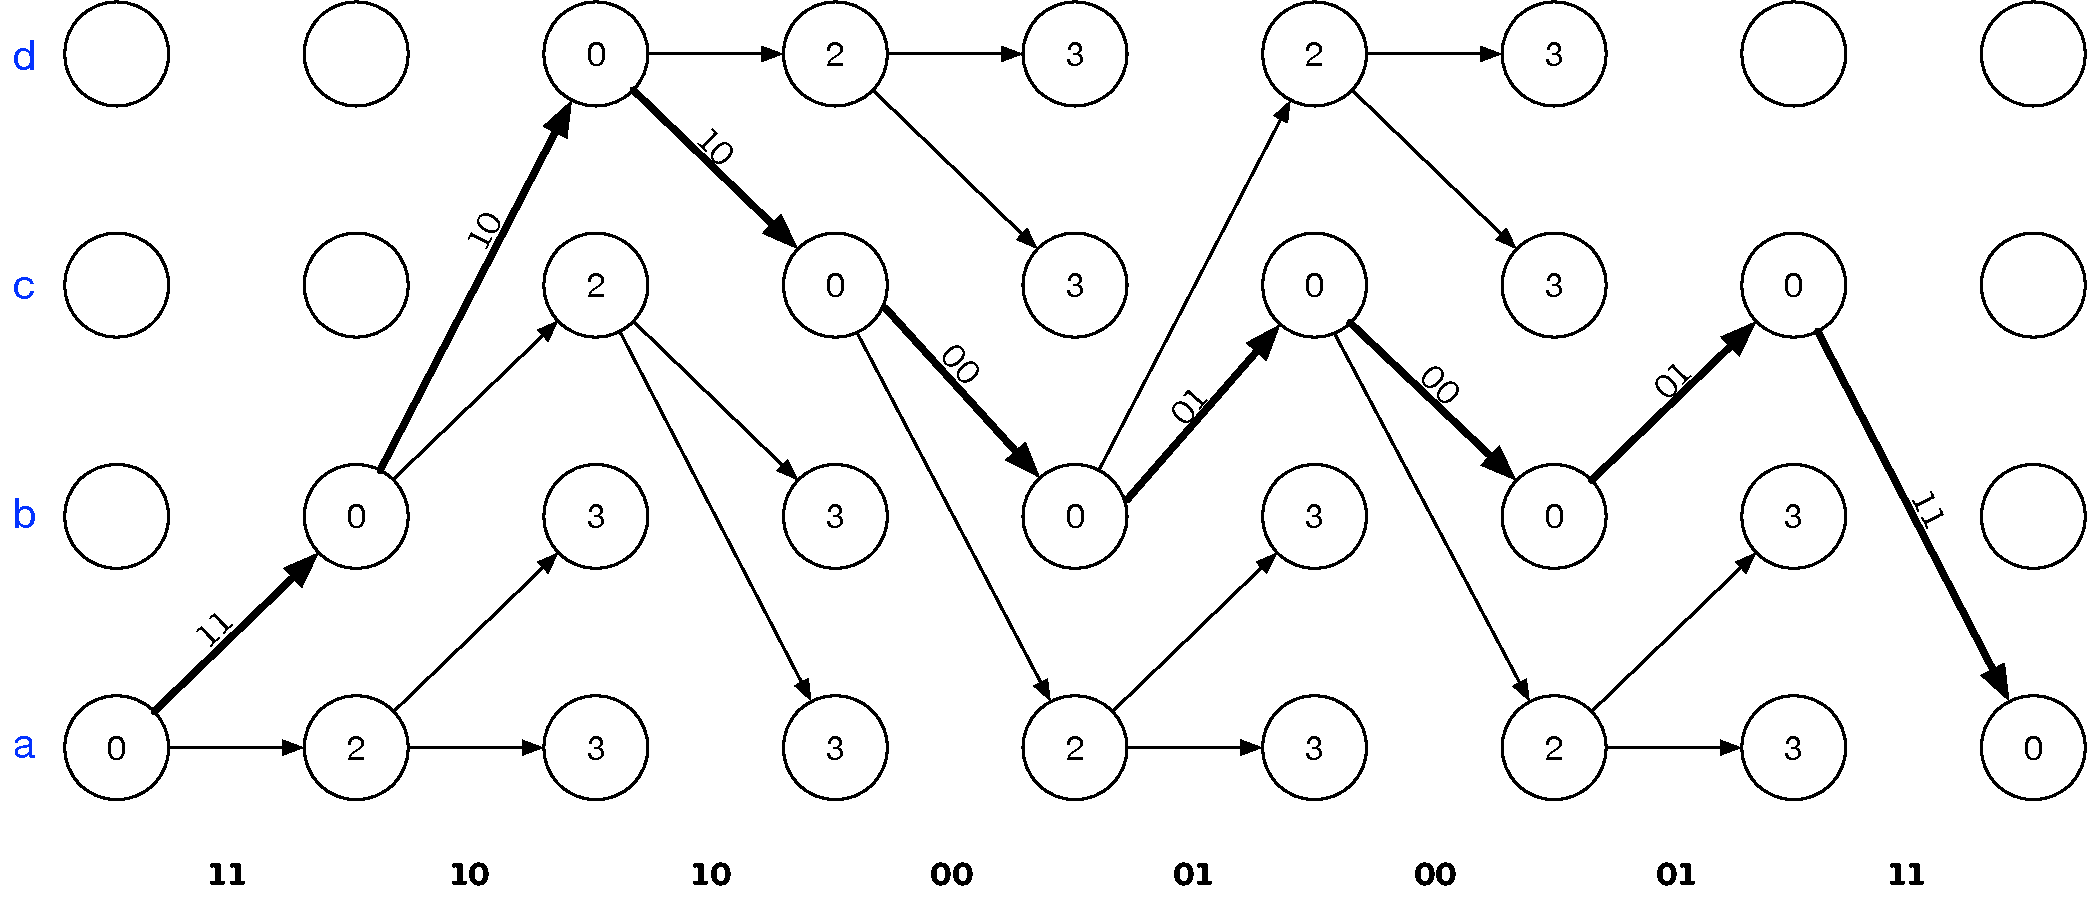
\includegraphics[width=10cm]{./Figuras/Viterbi_5}
		\caption{Resultado final del algoritmo de Viterbi.}	
		\label{fig:Viterbi_5}
\end{figure*}



\newpage

\section{Problemas propuestos}

%\begin{center}
%\noindent\rule{\linewidth}{0.4pt}
%\ \\
%\textrm{{\bf Ejercicios}} \\
%\end{center}

	


	\Problema{
		Para un código de repetición con $n=5$, y una probabilidad de error de bit $p_e = 10^{-3}$, calcule:
		\begin{enumerate}
			\item La eficiencia del codificador.
			\item La distancia mínima
			\item El número de errores que pueden ser detectados
			\item El número de errores que pueden ser corregidos.
			\item La probabilidad de que se produzca un error y no sea detectado.
			\item La probabilidad de que se produzca un error en la decodificación.
		\end{enumerate}
		

		\textsc{Nota}: Considere que $P(i,n) \approx \left ( \begin{array}{c}n \\i \end{array} \right ) \cdot p_e^i$

		}
		{
		\begin{enumerate}
			\item $R_c = 1/5$
			\item $d_{min} = 5$
			\item 4 errores
			\item 2 errores
			\item $p = 10^{-15}$
			\item $p \approx 10^{-8}$
		\end{enumerate}

		}
		{

		}{

		}	
	
	\Problema{
		Calcule la distancia Hamming entre la palabra \bits{0100101} y las siguientes palabras: \bits{0111111}, \bits{1010111} y \bits{1101000}.

		}
		{
		3, 4 y 4 respectivamente.\\

		}
		{

		}{

		}

	\Problema{Calcule la probabilidad de que una palabra tenga a) errores detectados b) errores no detectados y c) no tenga errores cuando usamos un código de paridad con $n=4$ y $p_e=0.1$.

		\textsc{Nota}: Considere que $P(i,n) = \left ( \begin{array}{c}n \\i \end{array} \right ) \cdot p_e^i \cdot (1-p_e)^{n-i}$}
		{
		\begin{enumerate}
			\item $p \approx 0.2916$
			\item $p \approx 0.0486$
			\item $p = 0.6561$ 
		\end{enumerate}
		}
		{}{}
	
	\Problema{Un código tiene las siguientes siete palabras código: \bits{0010}, \bits{0100}, \bits{1110}, \bits{1000}, \bits{1010}, \bits{1100}, \bits{0110}.
			¿Es lineal?}
		{No.\\}{}{}
		
	
	
	\Problema{Un código de repetición puede verse como un caso particular de un código bloque lineal. Para el caso $(4,1)$, ¿Cuáles serían sus matrices generadora y de comprobación de paridad?}
		{$G = (1 1 1 1)$\\}{}{}
	
	\Problema{La matriz de codificación de un código lineal Reed-Muller (3,1) es:
		\begin{displaymath}
			\mathbf{G} = \left ( \begin{array}{cccccccc}
				\mathtt{1} & \mathtt{1} & \mathtt{1} & \mathtt{1} & \mathtt{1} & \mathtt{1} & \mathtt{1} & \mathtt{1}\\
				\mathtt{0} & \mathtt{1} & \mathtt{0} & \mathtt{1} & \mathtt{0} & \mathtt{1} & \mathtt{0} & \mathtt{1}\\
				\mathtt{0} & \mathtt{0} & \mathtt{1} & \mathtt{1} & \mathtt{0} & \mathtt{0} & \mathtt{1} & \mathtt{1}\\
				\mathtt{0} & \mathtt{0} & \mathtt{0} & \mathtt{0} & \mathtt{1} & \mathtt{1} & \mathtt{1} & \mathtt{1}\\
			\end{array} \right )
		\end{displaymath}

		Determine la tasa del código, su distancia mínima y la tabla de síndromes.

		\textsc{Pista}: El cálculo de la tabla de síndromes es más sencillo si antes se transforma el código en uno sistemático.
		}
		{$R_c = 1/2$, $d_{min} = 4$
		\begin{center}
\begin{tabular}{cc}
\hline
		Error			& Síndrome 		\\	
	\hline
	\bits{00000001}	& \bits{0001}  \\
	\bits{00000010}	& \bits{0010}   \\
	\bits{00000100}	& \bits{0100}   \\
	\bits{00001000}	& \bits{1000} \\
	\bits{00010000}	& \bits{0111}   \\
	\bits{00100000}	& \bits{1011}  \\
	\bits{01000000}	& \bits{1101}   \\
	\bits{10000000}	& \bits{1110}   \\
\hline
\end{tabular}
\end{center}
}
{}{}

	\Problema{Dada la matriz generadora para un código lineal $(7,3)$:
		\begin{displaymath}
			\mathbf{G} = \left (
			\begin{array}{ccccccc}
				\mathtt{0} & \mathtt{0} & \mathtt{1} & \mathtt{1} & \mathtt{1} & \mathtt{0} & \mathtt{1} \\
				\mathtt{0} & \mathtt{1} & \mathtt{0} & \mathtt{0} & \mathtt{1} & \mathtt{1} & \mathtt{1} \\
				\mathtt{1} & \mathtt{0} & \mathtt{0} & \mathtt{1} & \mathtt{1} & \mathtt{1} & \mathtt{0} \\
			\end{array} \right )
		\end{displaymath}
		
		\begin{enumerate}
			\item Construya la matriz generadora de un código sistemático equivalente.
			\item Encuentre la matriz de control de paridad.
			\item Construya la tabla de síndromes
			\item Calcule la distancia mínima del código. ¿Qué capacidad correctora de errores tiene este código?
			\item Compare las prestaciones de este código con las de un Hamming $(7,4)$. ¿Existe alguna relación entre ambos?
			\item Calcule la palabra codificada cuando a la entrada tenemos al palabra \bits{101}. Verifique que su síndrome es $\mathbf{0}$.
			
		\end{enumerate}
		}
		{\begin{enumerate}
		\item $\mathbf{G} = \left (
			\begin{array}{ccccccc}
				\mathtt{1} & \mathtt{0} & \mathtt{0} & \mathtt{1} & \mathtt{1} & \mathtt{0} & \mathtt{1} \\
				\mathtt{0} & \mathtt{1} & \mathtt{0} & \mathtt{0} & \mathtt{1} & \mathtt{1} & \mathtt{1} \\
				\mathtt{0} & \mathtt{0} & \mathtt{1} & \mathtt{1} & \mathtt{1} & \mathtt{1} & \mathtt{0} \\
			\end{array} \right ) $
			
		\item $\mathbf{H} = \left (
			\begin{array}{ccccccc}
				\mathtt{1} & \mathtt{0} & \mathtt{1} & \mathtt{1} & \mathtt{0} & \mathtt{0} & \mathtt{0} \\
				\mathtt{1} & \mathtt{1} & \mathtt{1} & \mathtt{0} & \mathtt{1} & \mathtt{0} & \mathtt{0} \\
				\mathtt{0} & \mathtt{1} & \mathtt{1} & \mathtt{0} & \mathtt{0} & \mathtt{1} & \mathtt{0} \\
				\mathtt{1} & \mathtt{1} & \mathtt{0} & \mathtt{0} & \mathtt{0} & \mathtt{0} & \mathtt{1} \\
			\end{array} \right ) $
			\item 		
\begin{tabular}{ll}
	\bits{0000001} $\rightarrow$&\bits{0001}  \\
	\bits{0000010} $\rightarrow$&\bits{0010}   \\
	\bits{0000100} $\rightarrow$&\bits{0100}   \\
	\bits{0001000} $\rightarrow$&\bits{1000} \\
	\bits{0010000} $\rightarrow$&\bits{1110}   \\
	\bits{0100000} $\rightarrow$&\bits{0111}  \\
	\bits{1000000} $\rightarrow$&\bits{1101}   \\
\end{tabular}

			\item $d_{min} = 4 \Rightarrow $  Se pueden detectar hasta 3 errores y corregir 1 error.
			\item El Hamming tiene mayor eficiencia, puede corregir los mismos errores, pero sólo puede detectar 2.
			\item $\mathtt{101} \rightarrow \mathtt{1010011}$
		\end{enumerate}
		}
		{}{}
	

	\Problema{Construya el árbol y el diagrama de estados para un código convolucional $(3,1,3)$ definido por las siguientes ecuaciones:
		\begin{displaymath}
			\begin{array}{l}
				x'_j = m_j \\
				x''_j = m_{j-2} \oplus m_j \\
				x'''_j = m_{j-3} \oplus m_{j-1}
			\end{array}
		\end{displaymath}
		}
		{\begin{figure*}[h!]\centering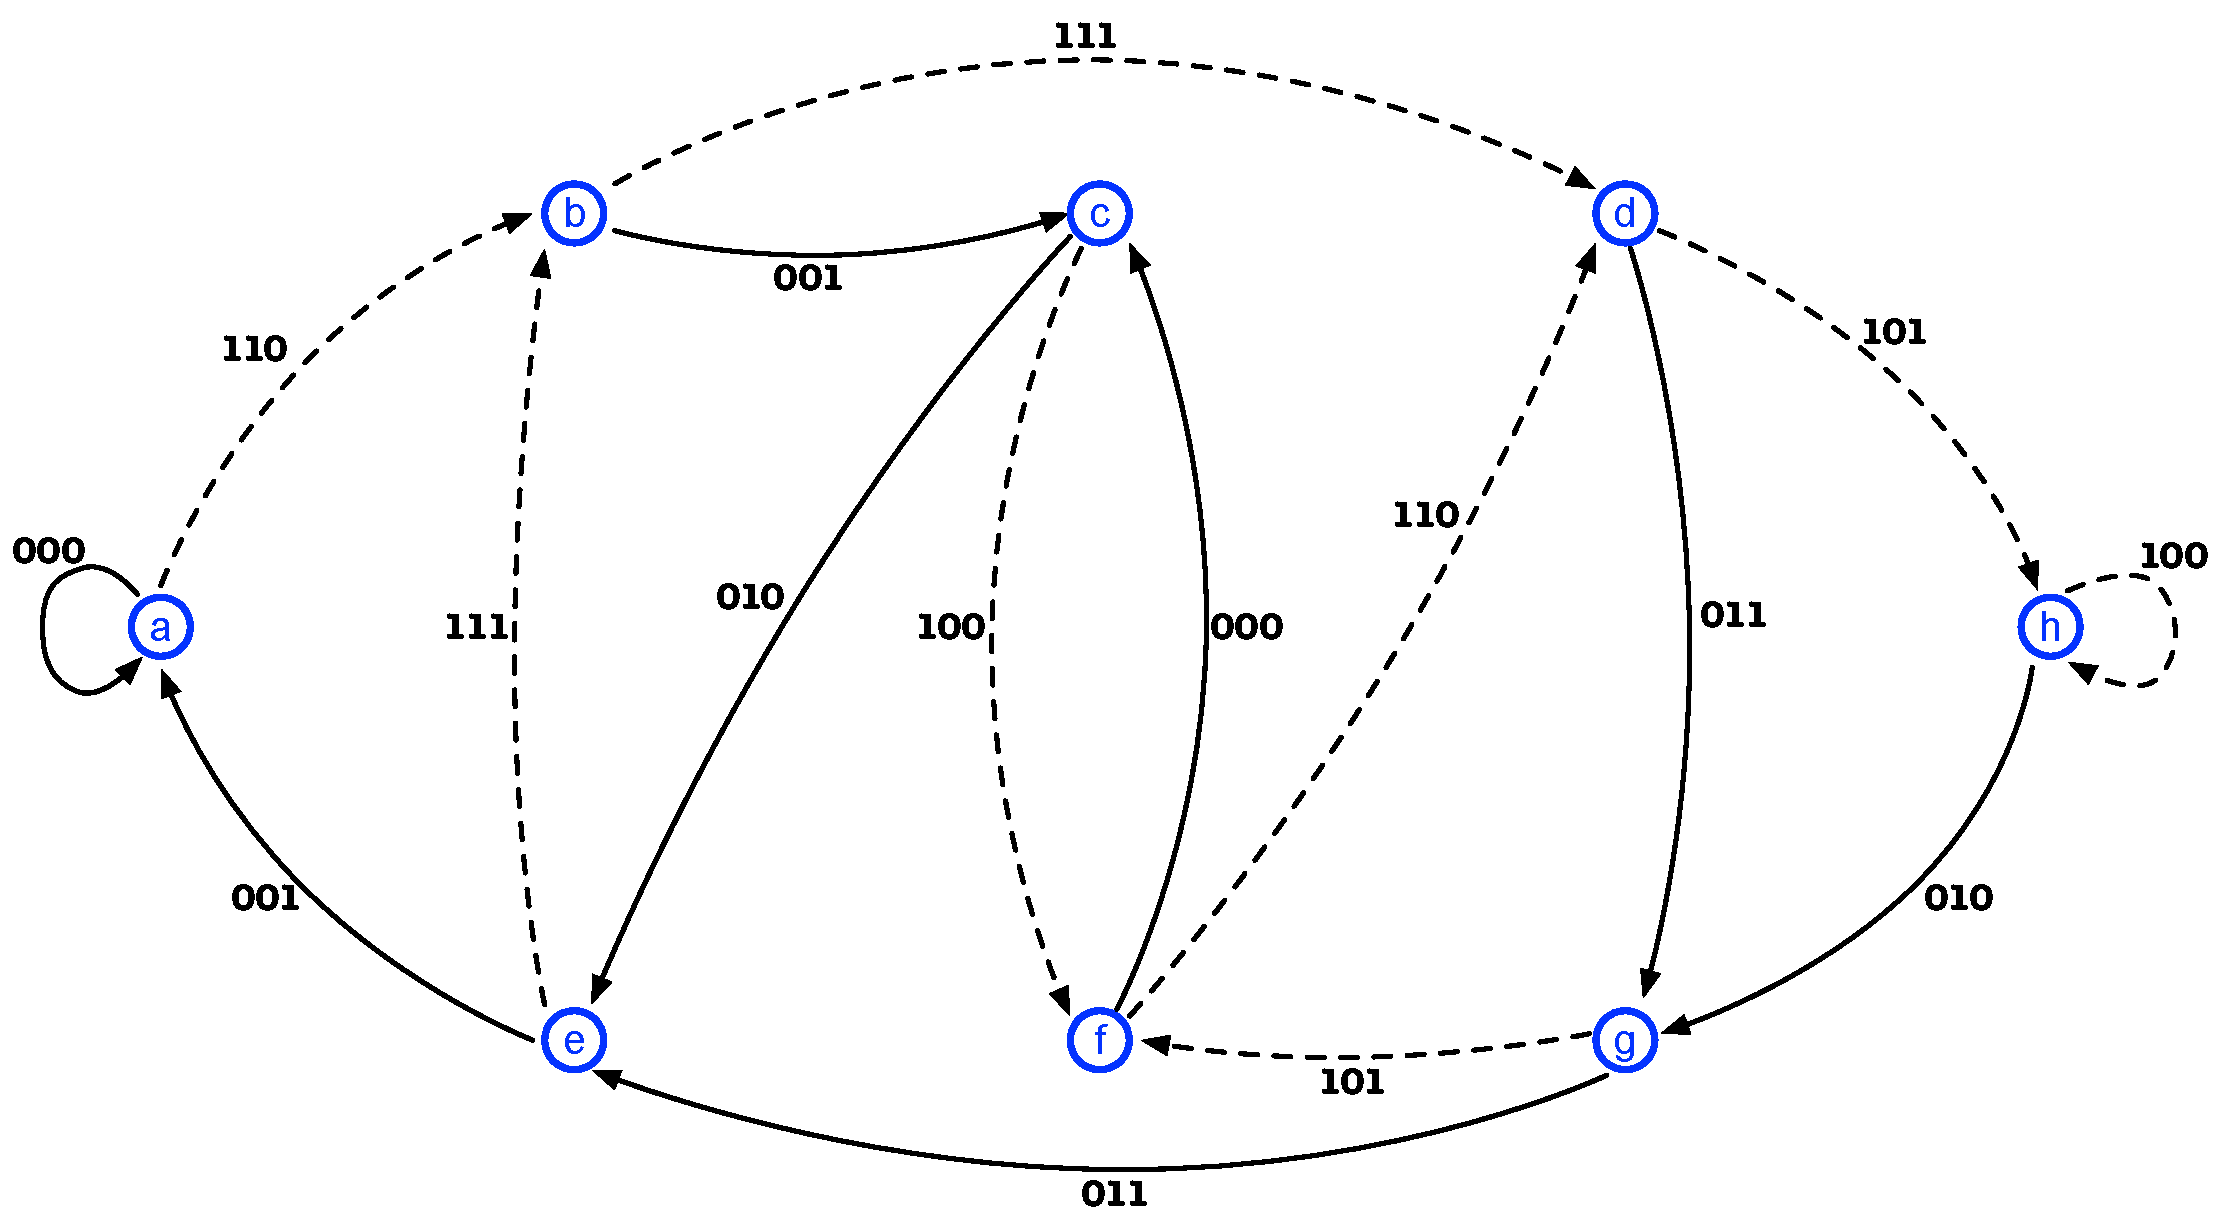
\includegraphics[width=6cm]{./Figuras/Ejercicio8_estados}\end{figure*} \ \\}
		{}{}

	\Problema{Considere un código convolucional de tasa $R_c = 1/2$ con matriz generadora $\mathbf{G} = \left [D \,\,\, D^2+1 \right]$. Dibuje su diagrama de estados y su diagrama de rejilla etiquetando cada transición con el bit de entrada y los dos bits de salida.
	}
	{
	\begin{figure}[h!]\centering
		\begin{subfigure}[]{}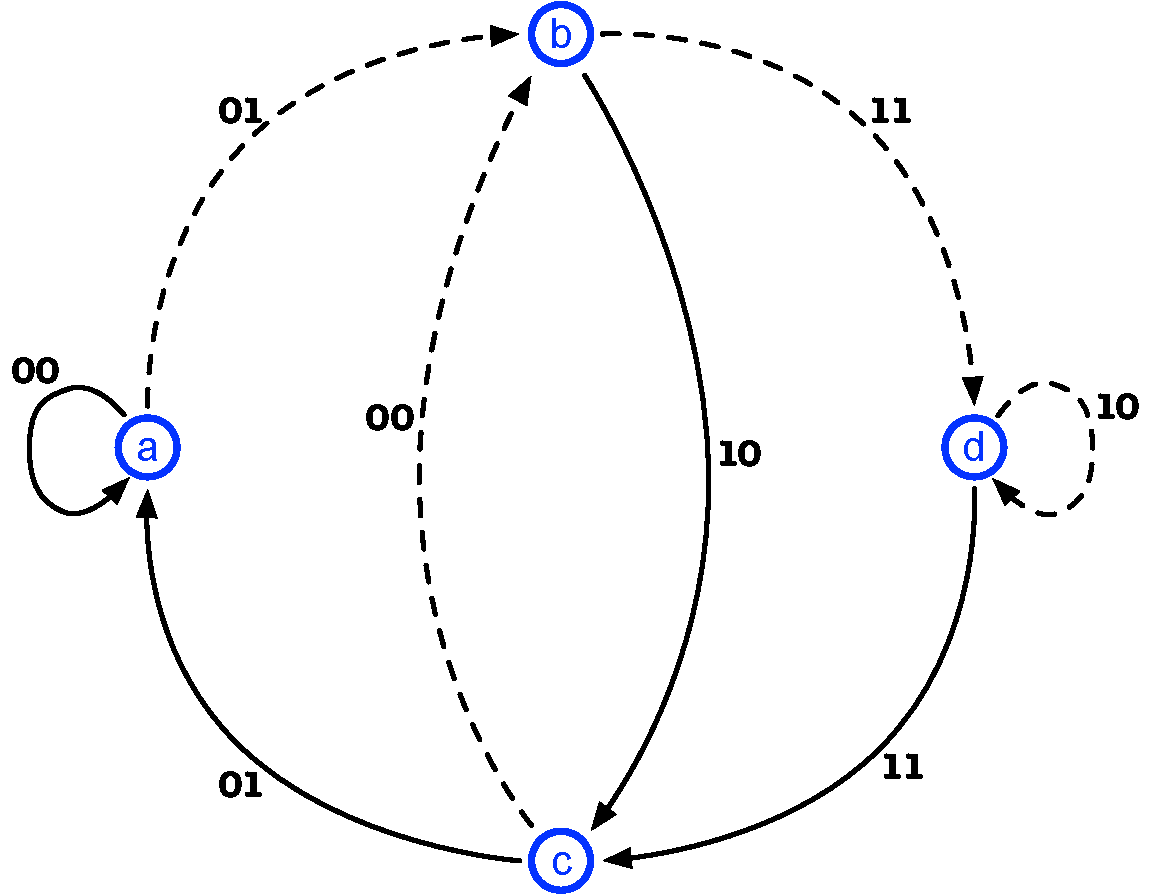
\includegraphics[width=4cm]{./Figuras/Ejercicio9_estados}\end{subfigure}
		\begin{subfigure}[]{}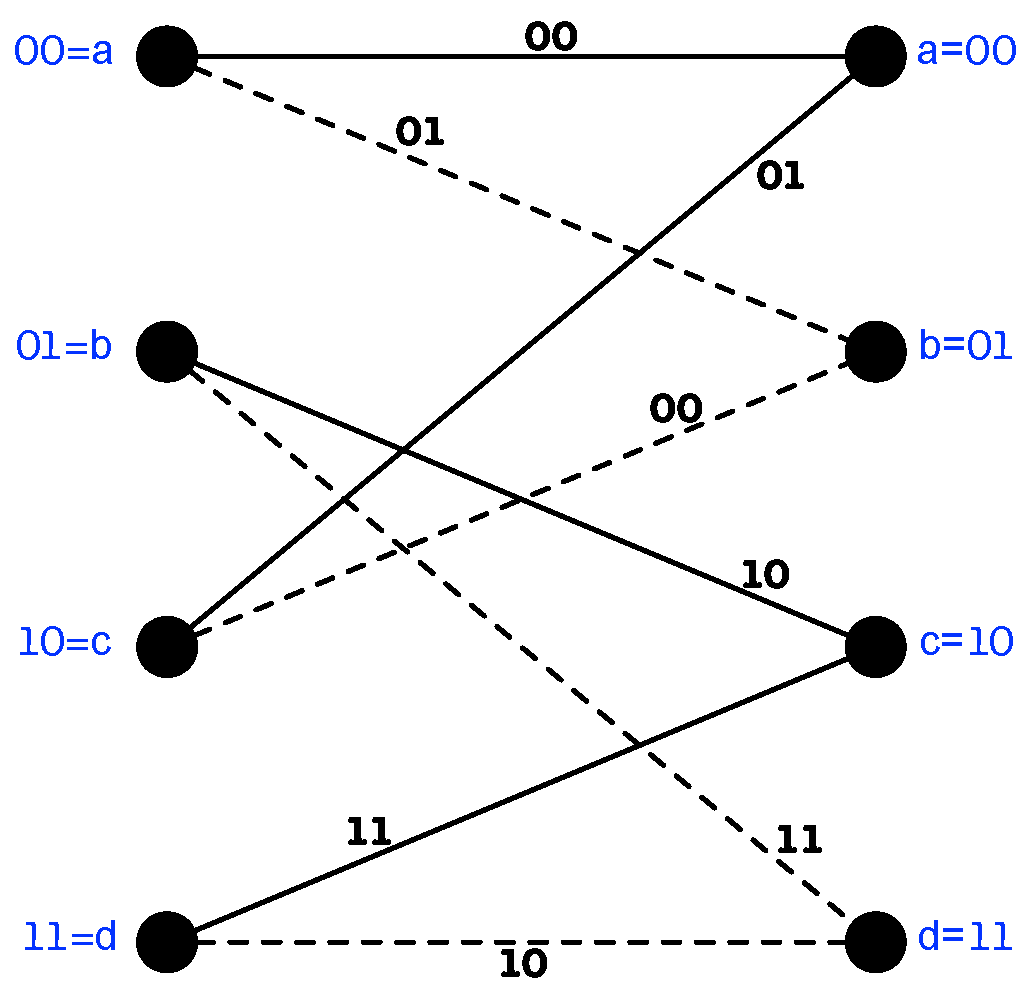
\includegraphics[width=4cm]{./Figuras/Ejercicio9_rejilla}\end{subfigure}
	\end{figure} \ \\
  }{}{}
	
	\Problema{Considere un código convolucional de tasa $R_c = 1/2$ con matriz generadora $\mathbf{G} = \left [1 \,\,\,\, D+1 \right]$. Dibuje su diagrama de estados y su diagrama de rejilla etiquetando cada transición con el bit de entrada y los dos bits de salida.}
	{\begin{figure}[h!]\centering
		\begin{subfigure}[]{}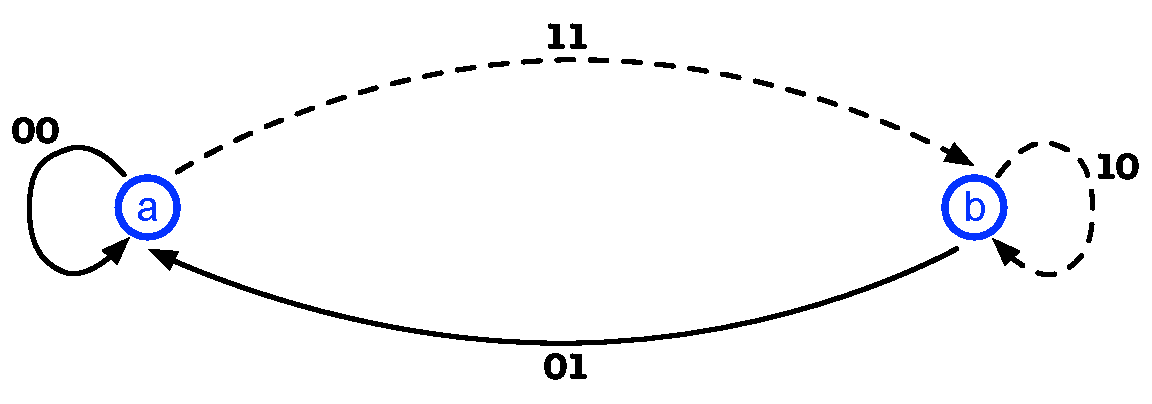
\includegraphics[width=4cm]{./Figuras/Ejercicio10_estados}\end{subfigure}
		\begin{subfigure}[]{}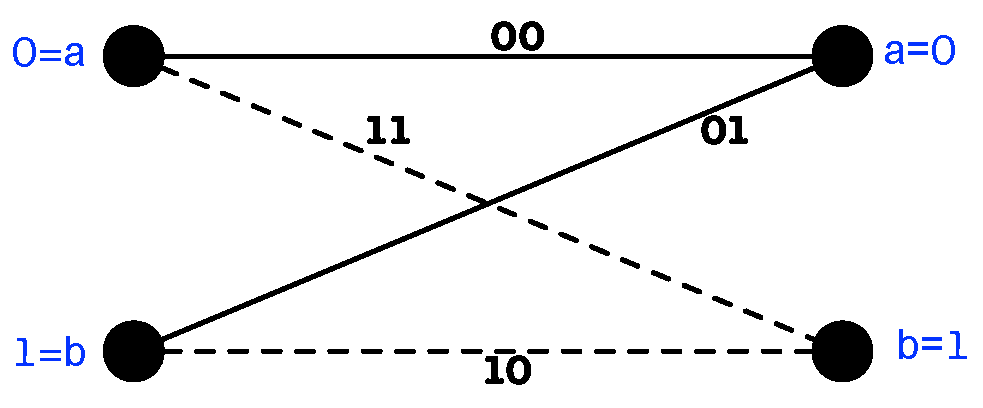
\includegraphics[width=4cm]{./Figuras/Ejercicio10_rejilla}\end{subfigure}
	\end{figure} \ \\}{}{}

		
	\Problema{Determine la salida del codificador $(3,2,1)$ de la figura para la entrada $(\mathtt{1101011101110000})$.
	\begin{figure*}[h!]
	\centering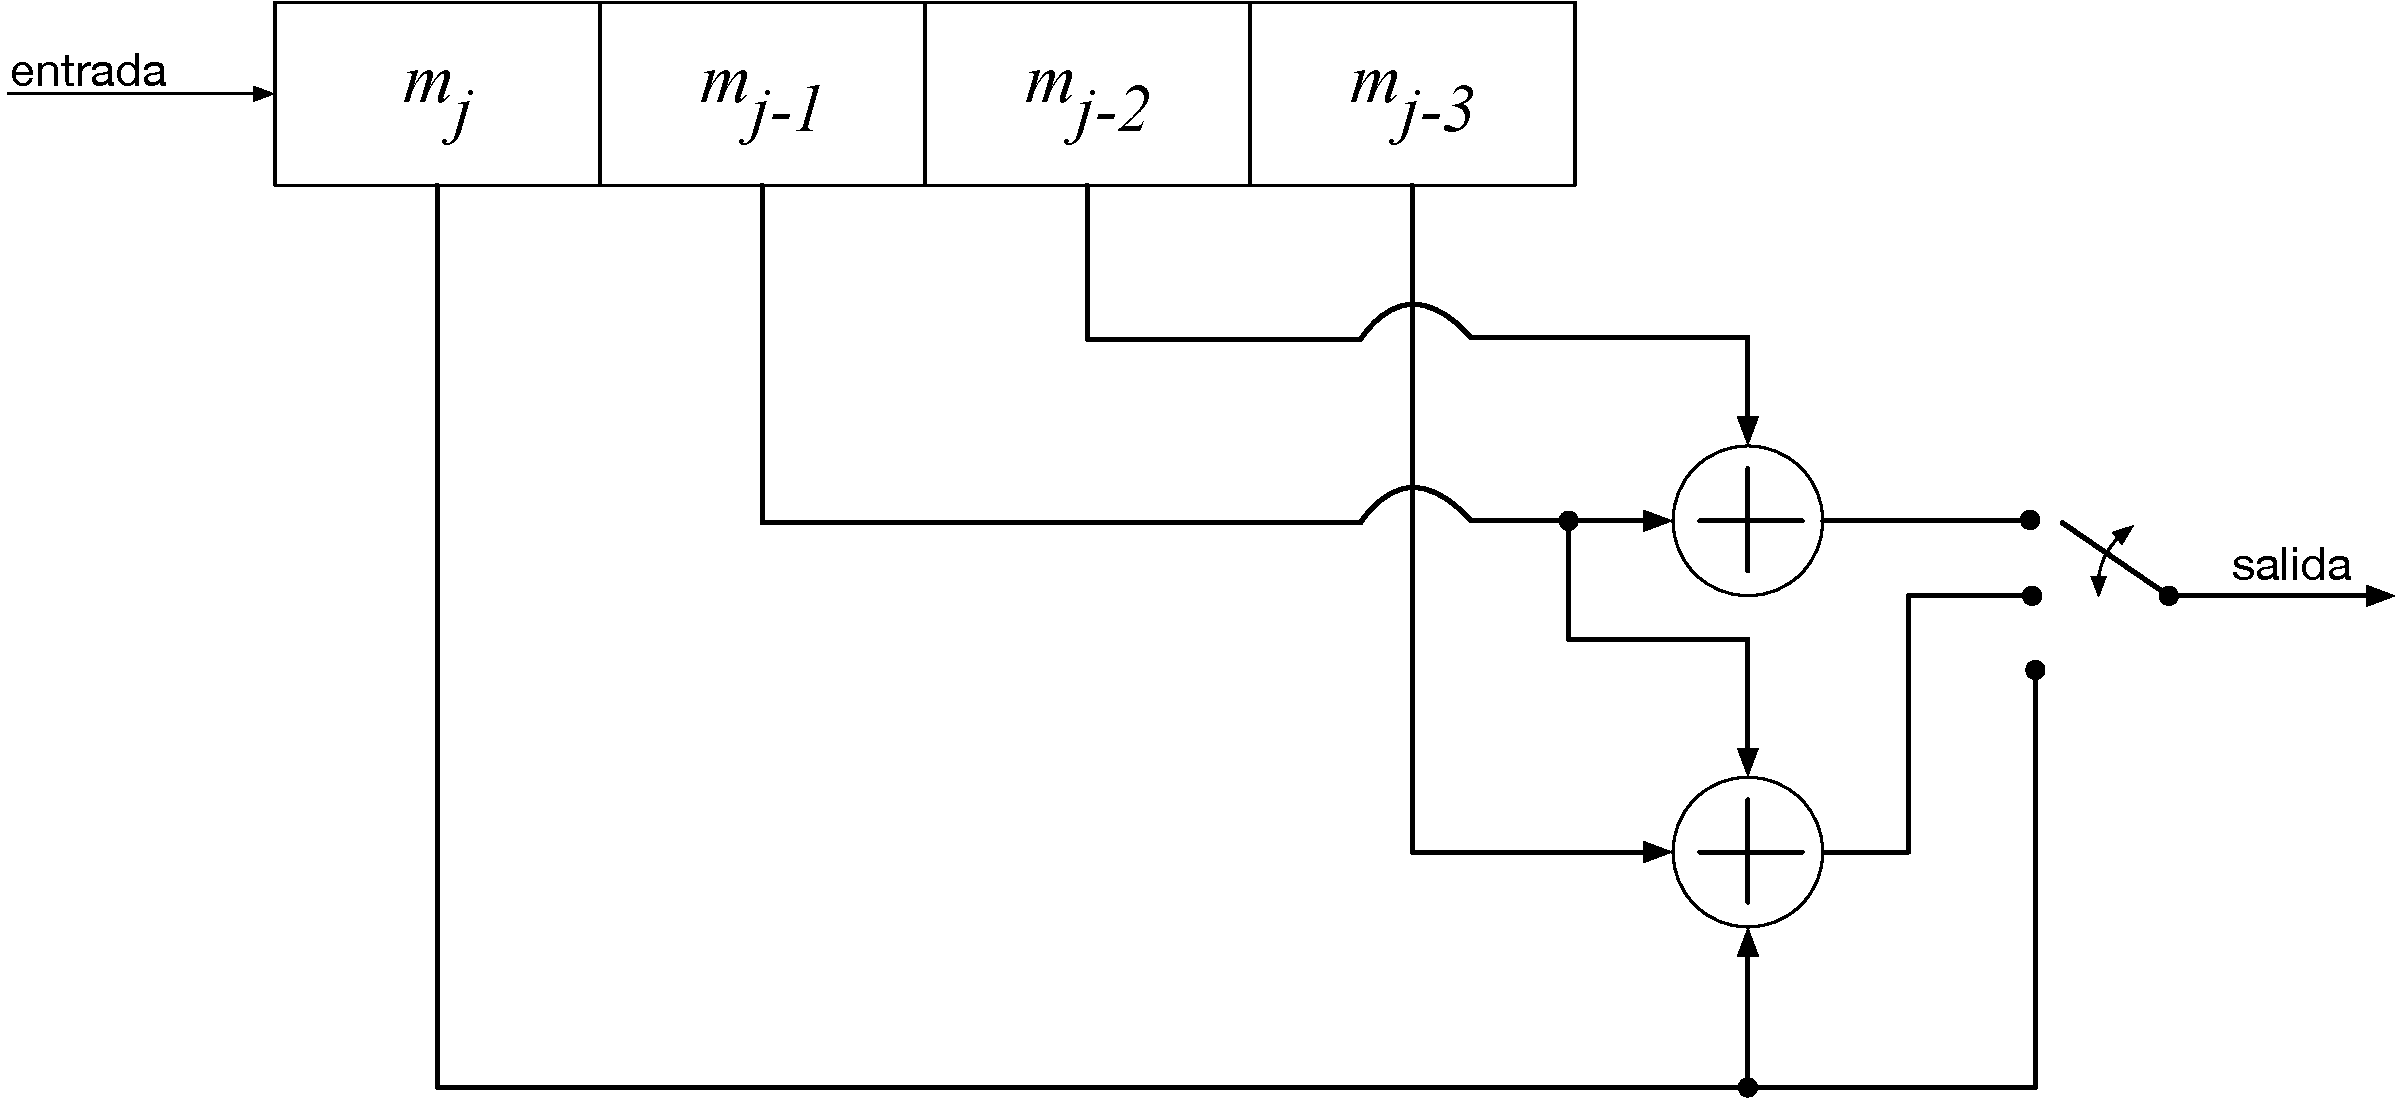
\includegraphics[width=7cm]{./Figuras/EjercicioConvolucionales}
	\label{fig:EjercicioConvolucionales}
	\end{figure*}
	}
	{$x_j' = m_{j-1} \oplus m_{j-2} = \bits{0101111001100100}$\\
	 $x_j'' = m_{j} \oplus m_{j-1} \oplus m_{j-3} = \bits{1010011000100110}$\\
	 $x_j''' = m_{j} = \bits{1101011101110000}$\\}{}{}
	
	
	\Problema{Para el codificador utilizado en los ejemplos del texto: 
	\begin{displaymath}
	\begin{array}{l}
		x'_j = m_j \oplus m_{j-2} \\
		x''_j = m_j \oplus m_{j-1} \oplus m_{j-2} \\
	\end{array}
\end{displaymath}

	 Obtenga, mediante el algoritmo de Viterbi, la secuencia decodificada siendo ahora la secuencia recibida: \\
	 \bits{10\,10\,10\,01\,01\,01\,01\,11}.
	 
	 }
	 {
		 \bits{11 10 10 00 01 00 01 11}\\}{}{}
	
	
	
	\Problema{Un código Golay (23,12) es un código perfecto capaz de corregir 3 errores. Este código se puede definir de forma cíclica mediante cualquiera de los siguientes polinomios generadores:
	\begin{displaymath}
		\begin{array}{l}
		g_1(x) = x^{11}+x^{10}+x^6+x^5+x^4+x^2+1 \\
		g_2(x) = x^{11}+x^9+x^7+x^6+x^5+x+1 \\
	\end{array}
	\end{displaymath}
	
	\begin{enumerate}
		\item Verifique que efectivamente se trata de un código perfecto. 
		\item Codifique la palabra $\mathbf{b} = [\bits{010001100001}]$ de forma sistemática empleando $g_1(x)$ y de forma directa multiplicando $b(x)$ por $g_2(x)$.
	\end{enumerate}
	.
	 }
	 {De forma sistemática: $\mathbf{c} = [\bits{11110000101010001100001}]$\\}{}{}
	
	



\end{document}



	
